% LaTeX Vorlage
%\documentclass[
%  ngerman,		% Sprache
%  a4paper,		% Papierformat
%  11pt,			% Schriftgröße (default 10pt)
%  DIV=12,		% Seiteneinteilung
%  parskip=half  	% Absätze (full,half,false -+*)
%]{scrartcl}
\documentclass{beamer}
%\documentclass[handout]{beamer}

\usepackage[status=draft]{fixme}
%\usepackage[status=final]{fixme}

\usepackage[utf8]{inputenc} % UTF-8
\usepackage[ngerman,english,main=english]{babel} % Sprache 
\selectlanguage{english}
\usepackage{amsmath, amssymb}
\usepackage{graphicx} % Grafiken einbinden
%\usepackage[left=2cm,right=2cm,top=2.5cm,bottom=3cm]{geometry}
\usepackage{color} % Farbe
\usepackage{bbm}
\usepackage{geometry}
\usepackage[absolute,overlay]{textpos}

\usetheme[height=10mm]{Rochester}
%\usetheme{Boadilla}
%\usetheme{ AnnArbor | Antibes | Bergen | Berkeley | Berlin | Boadilla | boxes | CambridgeUS | Copenhagen | Darmstadt | default | Dresden | 	Frankfurt | Goettingen |Hannover | Ilmenau | JuanLesPins | Luebeck | Madrid | Malmoe | Marburg | Montpellier | PaloAlto | Pittsburgh | Rochester | Singapore | Szeged | Warsaw }
\usecolortheme{whale}
%\usecolortheme{ albatross | beaver | beetle | crane | default | dolphin | dove | fly | lily | orchid | rose |seagull | seahorse | sidebartab |structure | whale | wolverine }
\usefonttheme{default}
%\usefonttheme{ default | professionalfonts | serif | structurebold | structureitalicserif | structuresmallcapsserif }

% Innere Themen spezifizieren die inneren Elemente wie Kopf-, Fußzeile, Sidebar usw. einer Folie.
\useinnertheme{rectangles}
% \useinnertheme{
% 	circles | default | inmargin |
% 	rectangles | rounded
% }

% Äußere Themen spezifizieren die Grenzen einer Folie und sagen ob und wo die inneren Elemente liegen.
% \useoutertheme{
% 	default | infolines | miniframes |
% 	shadow | sidebar | smoothbars |
% 	smoothtree | split | tree
% }

% Um halbtransparente Overlays auf seinen Folien zu haben, reicht es folgenden Schalter zu setzen:
% \setbeamercovered{transparent}

% Zum Abschalten der kleinen Navigationsleiste am unteren Rand reicht folgende Zeile aus:
% \beamertemplatenavigationsymbolsempty

% Seitenzahlen in Fußzeile einfügen
%\setbeamertemplate{footline}[frame number]
\usepackage{helvet} %Schriftart helvetica
\geometry{paperwidth=15cm,paperheight=10cm,left=1cm,right=1cm}
\definecolor{UniRot}{RGB}{165,30,55} %rote Farbe
\definecolor{UniGrau}{RGB}{195,195,195} %graue Farbe
\definecolor{UniGold}{RGB}{180,160,105} %goldene Farbe
\setbeamercolor{title}{fg=white}
\setbeamercolor{frametitle}{fg=white}
\setbeamercolor{structure}{fg=UniRot}
\setbeamercolor{author in footline}{fg=UniRot,bg=white}
\setbeamertemplate{navigation symbols}{} %Menüleiste aus
\defbeamertemplate*{footline}{} %footline-Format
{
 {\color{UniRot}\hrule}
 \vspace{0.1cm}
 \hspace*{0.1cm}
 {
\includegraphics[width=20mm, keepaspectratio=true]{template/logo.pdf}}
 \begin{beamercolorbox}[ht=2ex,leftskip=0.3cm,rightskip=2.5cm]{author in footline}
  \scriptsize
  Felix Hekhorn - NLO HQ structure function in DIS \hfill \insertframenumber{}/\inserttotalframenumber{}
  \vspace{0.15cm}
 \end{beamercolorbox}
 \vspace*{0.1cm}
}


% Um die Metainfomationen zu setzen die unter anderem für die Titelseite verwendet werden, kann man sich folgender Befehle bedienen:
\title{Next-to-Leading Order QCD Corrections to\\ Inclusive Heavy-Flavor Production in\\ Polarized Deep-Inelastic Scattering} % Titel des Vortrages
%\subject{Higgs-Mechanismus} % Setzt Thema in den PDF-Dokument-Eigenschaften
%\subtitle[Masseerzeugung]{oder warum das Photon auf Diät gesetzt wurde} % Untertitel

\author[F. Hekhorn and M. Stratmann]{\underline{Felix Hekhorn} and Marco Stratmann} % Autor festlegen
\institute{Institute for Theoretical Physics, University of Tübingen}
% \institute[IfI -- HU Berlin]{Institut für Informatik\\ Humboldt-Universität zu Berlin}
%     Angabe des Institutes
\date{March, 2018}
%\date[13.12.12]{13. Dezember 2012} % Datum der Präsentation, alternativ kann mittels \date{\today} auch das aktuelle Datum eingetragen werden.
% \logo{\pgfimage[width=2cm,height=2cm]{hulogo}}
%     Die Datei hulogo.pdf (bzw. hulogo.png, hulogo.jpg, hulogo.mps bei Verwendung von pdftex als Backend) als Logo auf allen Folien, hier mithilfe des Paketes pgf.
% \titlegraphic{\includegraphics[width=2cm,height=2cm]{hulogo}}
%     Die Datei hulogo.pdf (bzw. analog wie bei \logo auch entsprechendes Format) als Logo nur auf der Titelseite unter Verwendung des Paketes graphicx.

\usepackage{pgfpages}
%\pgfpagesuselayout{resize to}[a4paper,border shrink=5mm,landscape]
%\pgfpagesuselayout{2 on 1}[a4paper,border shrink=5mm]
%\pgfpagesuselayout{4 on 1}[a4paper,border shrink=5mm,landscape]
%\pgfpagesuselayout{8 on 1}[a4paper,border shrink=5mm]
%\pgfpagesuselayout{16 on 1}[a4paper,border shrink=5mm,landscape]

%\usepackage{pdflscape}

\usepackage{wrapfig}
\usepackage{graphicx}
\usepackage{pdflscape}
\usepackage{ulem}
\usepackage{url}
\usepackage{caption}
\usepackage{subcaption}
\usepackage{array}
\usepackage{multirow}
%\usepackage{enumitem}
\usepackage{listings}
\usepackage{placeins}
\usepackage{csquotes}

\usepackage{siunitx} % SI Einheiten
\usepackage[version=3]{mhchem}
\usepackage{slashed}
\usepackage{hepnames}

\usepackage{url}
\usepackage{hyperref}
%\hypersetup{colorlinks=false}
\usepackage{tabularx}

\providecommand{\abs}[1]{\left|#1\right|}
\providecommand{\VektorV}[3]{
\!\left(\!\!
\begin{array}{c}
#1 \\ #2 \\ #3
\end{array}\!\!
\right)\!
}

\providecommand{\Det}[9]{
	\begin{vmatrix}
	    #1 & #2 & #3 \\
	    #4 & #5 & #6 \\
	    #7 & #8 & #9 \\	    
	\end{vmatrix}
}

\DeclareMathOperator{\Grad}{\text{grad}}
\DeclareMathOperator{\Div}{\text{div}}
\DeclareMathOperator{\Rot}{\text{rot}}
\DeclareMathOperator{\tr}{\text{tr}}

\DeclareMathOperator{\acos}{\text{arccos}}
\DeclareMathOperator{\asin}{\text{arcsin}}
\DeclareMathOperator{\atanh}{\text{artanh}}
\DeclareMathOperator{\DiLog}{\text{Li}_2}
\DeclareMathOperator{\x}{\times}
\DeclareMathOperator{\cdt}{\!\cdot\!}
\DeclareMathOperator{\del}{\partial}
\DeclareMathOperator{\EqualClaim}{\stackrel{!}{=}}
\DeclareMathOperator{\equivals}{\mathrel{\widehat{=}}}
\providecommand{\Nabla}[0]{\vec\nabla}
\providecommand{\ex}[1]{e^{#1}}
\providecommand{\EE}[1]{\cdot 10^{#1}}
\providecommand{\FT}[1]{\mathcal{FT}\left[#1\right]}
\providecommand{\Mel}[1]{\mathcal{M}\left[#1\right]}
\providecommand{\invMel}[1]{\mathcal{M}^{-1}\left[#1\right]}

\providecommand{\dt}[0]{\Derive t}
\providecommand{\dx}[0]{\Derive x}
\providecommand{\Derive}[1]{\DeriveN{#1}{}}
\providecommand{\DeriveN}[2]{\DeriveNF {#1}{#2}{}}
\providecommand{\DeriveF}[2]{\DeriveNF {#1}{}{#2}}
\providecommand{\DeriveNF}[3]{\frac {d^{#2}#3} {d #1^{#2}}}
\providecommand{\dtP}[0]{\DeriveP t}
\providecommand{\dxP}[0]{\DeriveP x}
\providecommand{\DeriveP}[1]{\DerivePN{#1}{}}
\providecommand{\DerivePF}[2]{\DerivePNF {#1} {} {#2}}
\providecommand{\DerivePN}[2]{\DerivePNF {#1} {#2} {} }
\providecommand{\DerivePNF}[3]{\frac {\partial^{#2}#3} {\partial #1^{#2}}}
\providecommand{\DerivePMF}[3]{\frac {\partial^{2}#3} {\partial #1 \partial #2}}
\providecommand{\e}[1]{\hat{e}_{#1}}
\providecommand{\pFq}[2]{{}_{#1}F_{#2}}

\providecommand{\bra}[1]{\langle#1\rvert}
\providecommand{\ket}[1]{\lvert#1\rangle}
\providecommand{\bracket}[2]{\langle#1\vert#2\rangle}
\providecommand{\normOrd}[1]{\,:\!#1\!:\,}
\providecommand{\wContr}[3]{\contraction{}{#1}{#2}{#3}#1#2#3}

\DeclareMathOperator{\Md}{\mathcal M}
\DeclareMathOperator{\Ld}{\mathcal L}
\DeclareMathOperator{\Hd}{\mathcal H}
\DeclareMathOperator{\Nd}{\hat {\mathcal N}}
\DeclareMathOperator{\To}{\hat {\mathcal T}}

\DeclareMathOperator{\MSbar}{\overline{\text{MS}}}

\DeclareRobustCommand{\PQ}{\HepGenParticle{Q}{}{}\xspace} % heavy quark
\DeclareRobustCommand{\PaQ}{\HepGenAntiParticle{Q}{}{}\xspace} % heavy anti-quark

\def\MMa{{\texttt{Mathematica}}}
\def\HEPMath{\texttt{HEPMath}}
\def\FeynCalc{\texttt{FeynCalc}}
\def\LoopTools{\texttt{LoopTools}}
\def\QCDLoop{\texttt{QCDLoop}}


\begin{document}

\frame[plain]{ \titlepage }
\frame{
	\frametitle{Outline}
	\tableofcontents
}

\fxerror{write intro}

\subsection{Motivation}
\fxerror{write motivation}

\subsection{Notation}
To collect all soft and collinear poles we have to calculate in $n=4+\epsilon$ dimension. Unfortunaly the extension for \textit{polarized} processes is nontrivial, because the occuring Levi-Civita tensors $\varepsilon_{\mu\nu\rho\sigma}$ and $\gamma_5$. A common choice to deal with these objects is the HVBM prescription\cite{breitenlohner1977} that keeps those two objects four dimensional at the price for splitting the full $n$ dimensional space into a $n-4$ dimensional space, called \enquote{hat-space}, and a four dimensional space (that is actually never used).

In leading order (LO) we have to consider the following processes
\begin{equation}
\Pggx(q;\sigma_q) + \Pg(k_1;\sigma_{k_1}) \rightarrow \PQ(p_1)+\PaQ(p_2)
\end{equation}
The corresponding parton structure tensor $W_{\mu\mu'}^{(0)}$ can then be written as
\fxerror{avoid all order expr?}
\begin{align}
&W_{\mu\mu'}^{(0)}(k_1,q;s,t_1,u_1,q^2;\sigma_{k_1}\sigma_{q})\nonumber\\
 &= \frac 1 2 E_\epsilon K_{\Pgg\Pg}\!\int\!\frac{d^{n-1}p_1}{2E_1(2\pi)^{n-1}}\!\int\!\frac{d^{n-1}p_2}{2E_2(2\pi)^{n-1}}\delta(p_1^2-m^2) \delta(p_2^2-m^2)\nonumber\\
 &\hspace{20pt}(2\pi)^n\delta^{(n)}(k_1+q-p_1-p_2) \Md_{\mu}^{(0)}(\sigma_{k_1})\Md_{\mu'}^{(0)}(\sigma_q)
\end{align}
where the initial $1/2$ is the initial state spin average, $K_{\Pgg\Pg}$ is the color average,
\begin{align}
E_\epsilon := \left\{\begin{array}{ll}
1/(1+\epsilon/2) &\text{unpolarized}\\
1 &\text{polarized}
\end{array}\right.
\end{align}
accounts for initial freedom in $n$ dimensions for bosons and we defined the following Mandelstam variables:
\begin{equation}
s = (q+k_1)^2, \quad t_1=t-m^2=(k_1-p_2)^2-m^2, \quad u_1 = u - m^2 = (q-p_2)^2 -m^2
\end{equation}
\begin{equation}
s' = s-q^2,\quad u_1' = u_1 - q^2
\end{equation}
\fxerror{move to LO?}
The Lorentz indices $\mu$ and $\mu'$ refer to the virtual photon that is exchanged with the scattering lepton.

By using Lorentz covariance, hermiticity, parity invariance and current conservation the parton structure tensor can be decomposed into several parts:
\begin{align}
W_{\mu\mu'}^{(0)}(k_1,q;s,t_1,u_1,q^2;\sigma_{k_1},\sigma_{q}) &= \left(-g_{\mu\mu'} + \frac{q_\mu q_{\mu'}}{q^2}\right)\frac{d^2\sigma_T(s,t_1,u_1,q^2)}{dt_1du_1} \nonumber\\
 &\hspace{20pt} +\left(k_{1,\mu}-\frac{k_1\cdot q}{q^2}q_\mu\right)\left(k_{1,\mu'}-\frac{k_1\cdot q}{q^2}q_{\mu'}\right)\left(\frac{-4q^2}{{s'}^2}\right) \nonumber\\
 &\hspace{30pt} \cdot\left(\frac{d^2\sigma_T(s,t_1,u_1,q^2)}{dt_1du_1}+\frac{d^2\sigma_L(s,t_1,u_1,q^2)}{dt_1du_1}\right)
\end{align}
\fxerror{extend}
We can then define appropiate projection operators\cite{Vogelsang:1993eg}:
\begin{align}
\mathcal P_{G,\mu\mu'} &= -g_{\mu\mu'} &b_G(\epsilon) &= \frac 1 {2(1+\epsilon/2)}\\
\mathcal P_{L,\mu\mu'} &= -\frac{4q^2}{{s'}^2} k_{1,\mu}k_{1,\mu'} &b_L(\epsilon) &= 1\\
\mathcal P_{P,\mu\mu'} &= i\varepsilon_{\mu\mu'\rho\rho'}\frac{q^{\rho}k_1^{\rho'}}{s'} &b_P(\epsilon) &= 1
\end{align}
\fxerror{justify avoidance of $\Delta$?}
\begin{align}
\frac{d^2\sigma_{k}(s,t_1,u_1,q^2)}{dt_1tu_1} &= b_k(\epsilon)\mathcal P_{k,\mu\mu'}W^{\mu\mu'}
\end{align}
with $k\in\{G,L,P\}$ denoting (here and mostly ever after) the projection type. The transverse partonic cross section $d\sigma_T$ can be reconstructed from the above definitions by using
\begin{align}
\frac{d^2\sigma_T}{dt_1du_1} &= \frac{d^2\sigma_G}{dt_1du_1} + b_G(\epsilon)\frac{d^2\sigma_L}{dt_1du_1}
\end{align}

\fxerror{explain ghosts?}

\fxerror{more}



\section{Computation Review}
\begin{frame}{Computation Review}
\begin{itemize}
\item use factorisation theorem: $s\to \xi S_h$ + PDF
\item $\Pg(k_1) + \Pggx(q) \to \PaQ(p_2) + \PQ(p_1)$
\item three massive particles: $2\cdot m^2>0,q^2=-Q^2<0$
\item compute 2-to-3-phase space: e.g. $dPS_3 \sim dt_1ds_4d\theta_1d\theta_2$
\item compute diagrams: 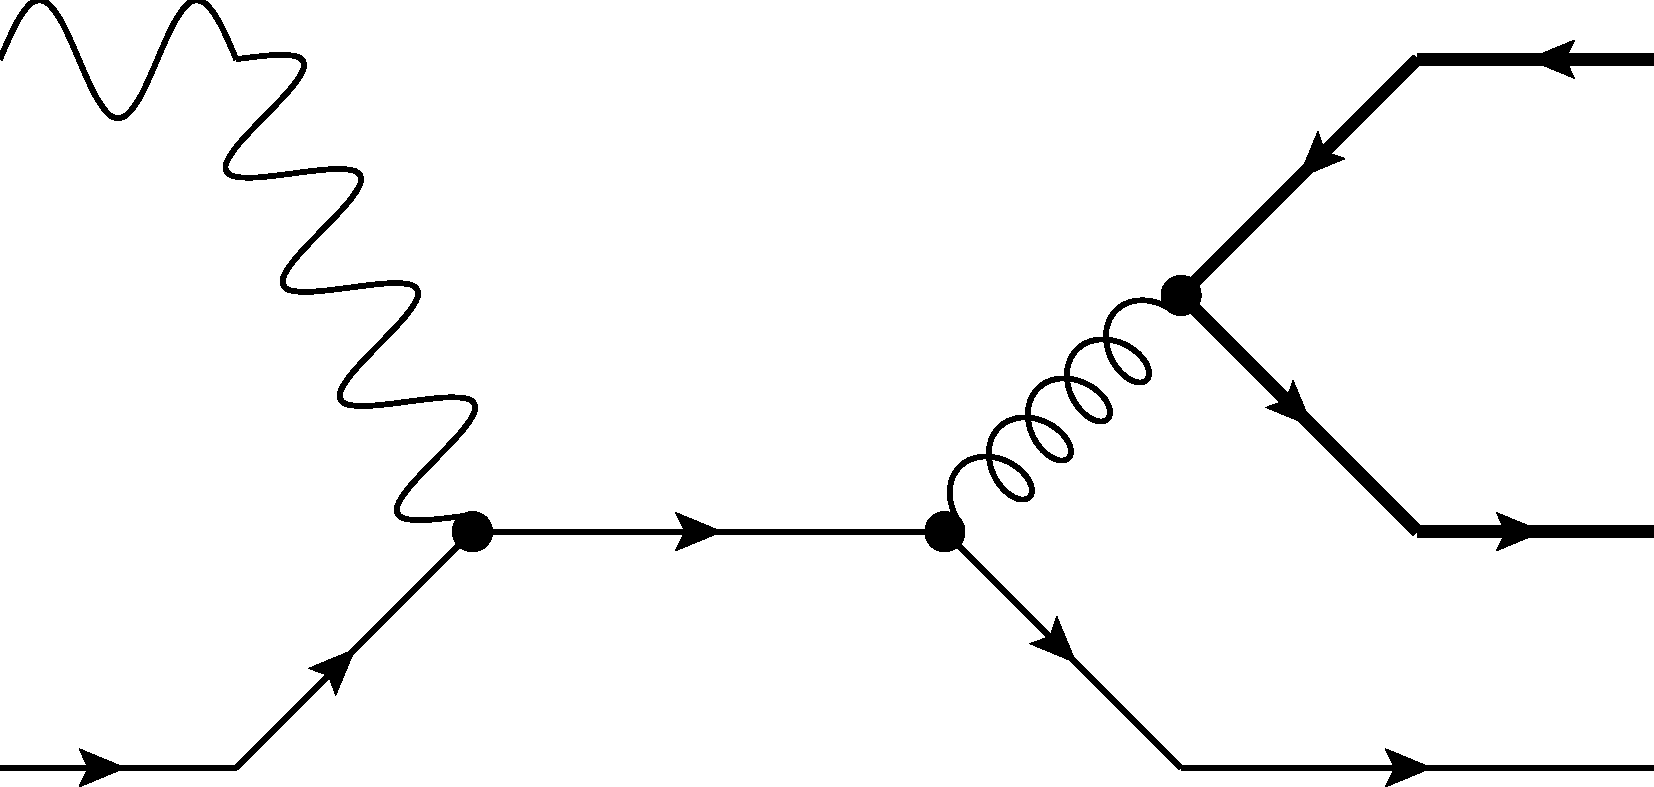
\includegraphics[width=.2\textwidth]{pyfeyn2/nlo-q-4} + 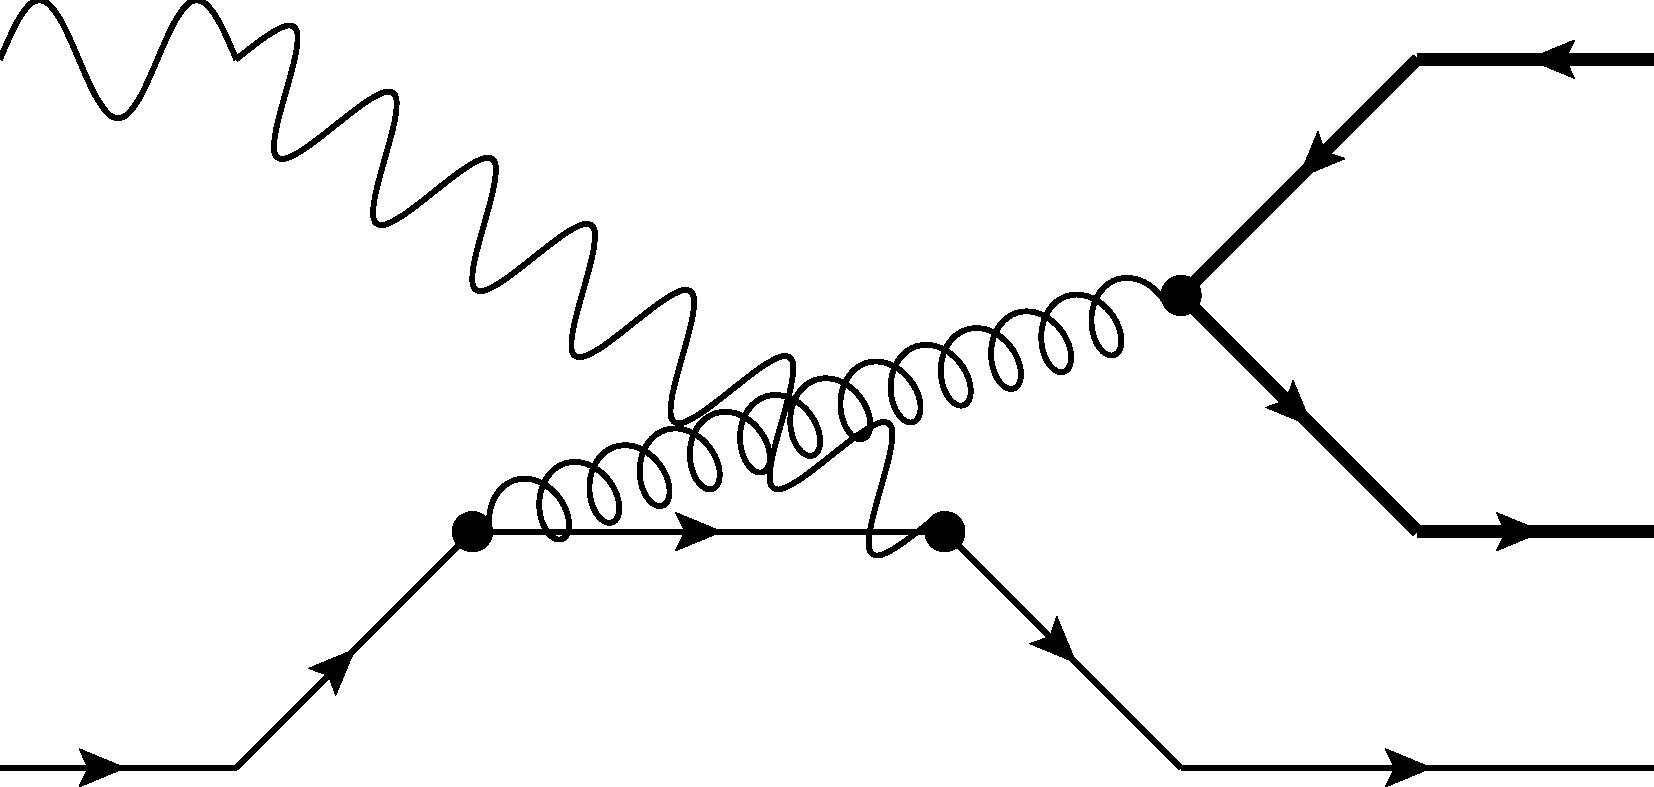
\includegraphics[width=.2\textwidth]{pyfeyn2/nlo-q-3}
\item $\Rightarrow 2xg_1(x) \sim e_u^2\cdot \xi\Delta f_u(\xi) \otimes d_{P,q}^{(1)}(\chi,\chi')$
\item $d_{P,q}^{(1)}(\chi,\chi') = c_1(\chi,\chi')\ln(\chi) + c_2(\chi,\chi')\DiLog\left(\frac{1+\chi'}{1+\chi}\right)+\ldots$ \checkmark
\item $\frac{m^2}{s} = \frac{\chi}{(1+\chi)^2}$ and $\frac{m^2}{s+Q^2} = \frac{m^2}{s'} = \frac{\chi'}{(1+\chi')^2}$ and $\frac{m^2}{Q^2} = \frac{\chi_q}{(1-\chi_q)^2}$
\end{itemize}
\end{frame}


\newcolumntype{w}{>{\centering\arraybackslash} m{.3\linewidth} }
\newcolumntype{n}{>{\centering\arraybackslash} m{.1\linewidth} }
\begin{frame}{Computation Review - Collinear Poles}
collinear poles appear as $1/\epsilon$ in
\begin{center}
\begin{tabular}{wnw}
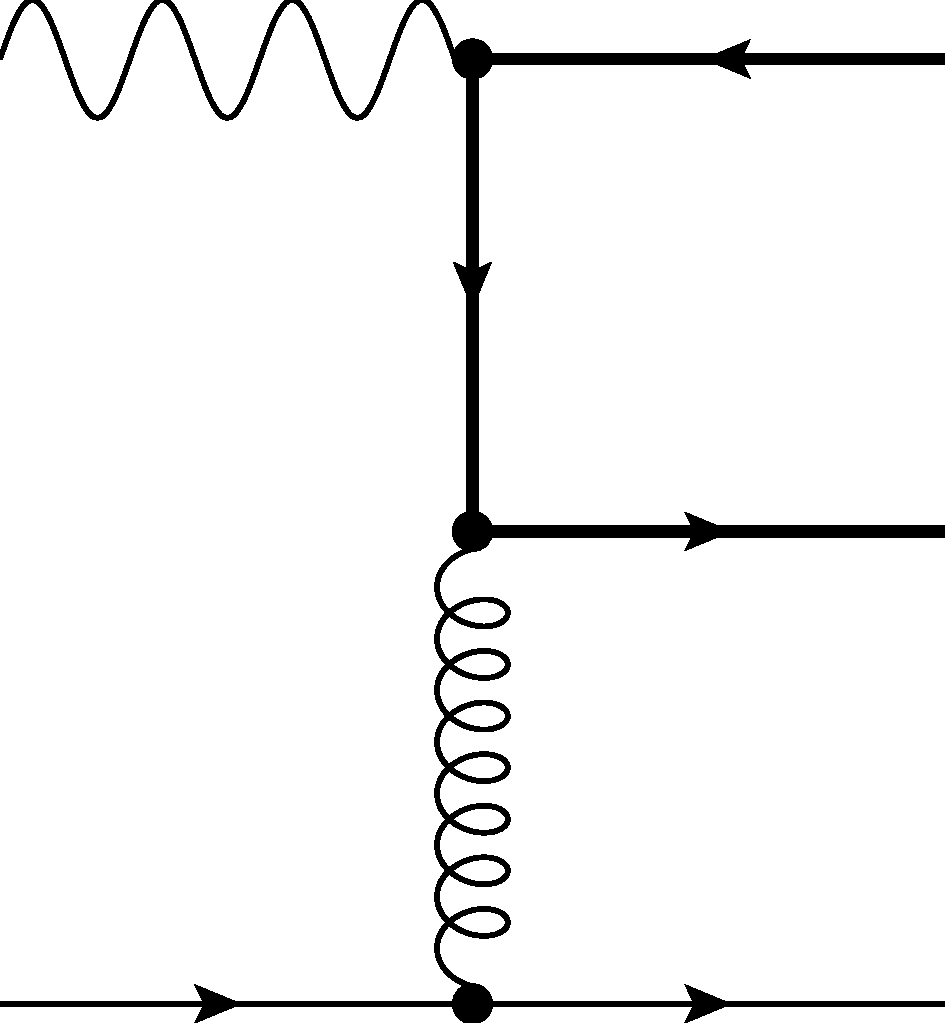
\includegraphics[width=.3\textwidth]{pyfeyn2/nlo-q-1}
&or
&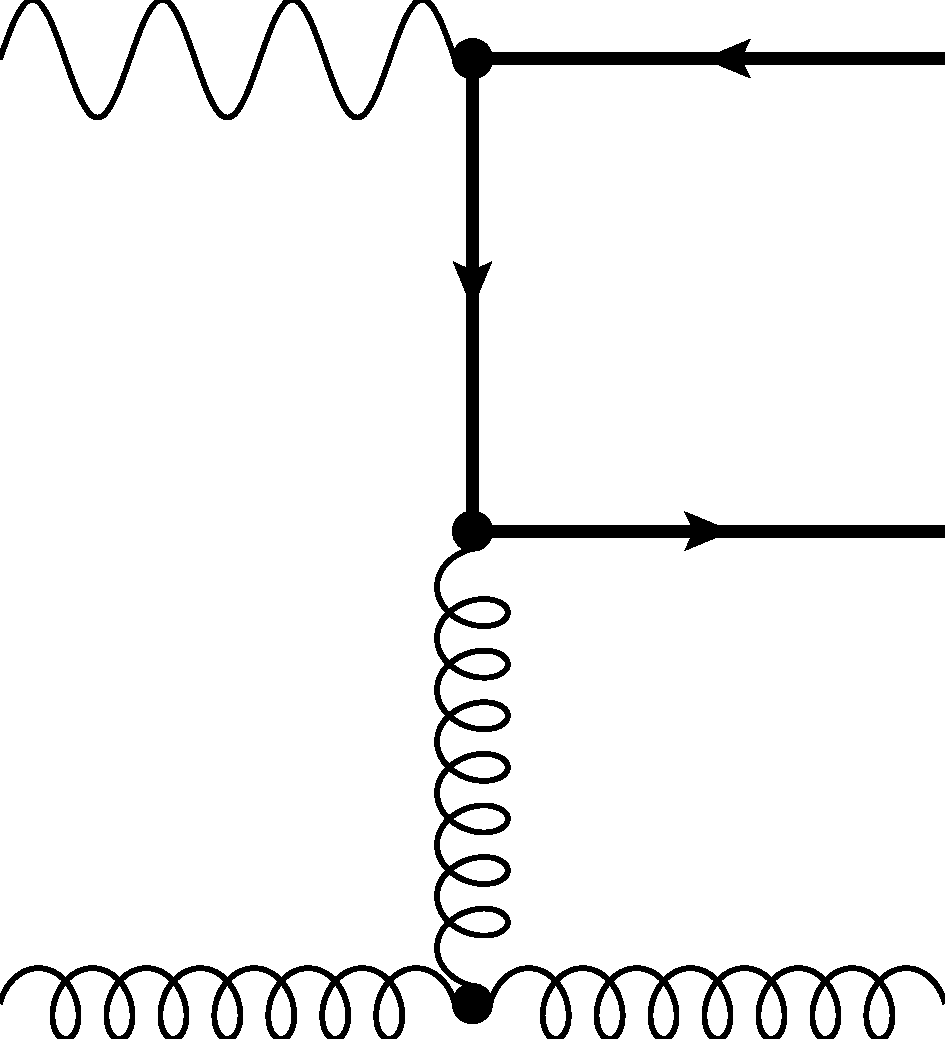
\includegraphics[width=.3\textwidth]{pyfeyn2/nlo-g-4}
\end{tabular}
\end{center}

\begin{itemize}
\item remove by mass factorization $\to \MSbar_m$
\item $\Rightarrow 2xg_1(x) \sim e_H^2\cdot \xi\Delta g(\xi) \otimes \ln(\mu_F^2/m^2) \bar c_{P,g}^{F,(1)}(\chi,\chi_q)$
\item $\bar c_{P,g}^{F,(1)}(\chi,\chi_q) = c_1(\chi,\chi_q)\ln(\chi) + c_2(\chi,\chi_q)\DiLog\left(\frac{1-\chi_q}{1+\chi}\right) + \ldots$ (\checkmark for $Q^2\gg m^2$ )
\end{itemize}
\end{frame}

\begin{frame}{Computation Review - Virtual and Soft Poles}
virtual diagrams are, e.g.,
\begin{center}
\begin{tabular}{wnw}
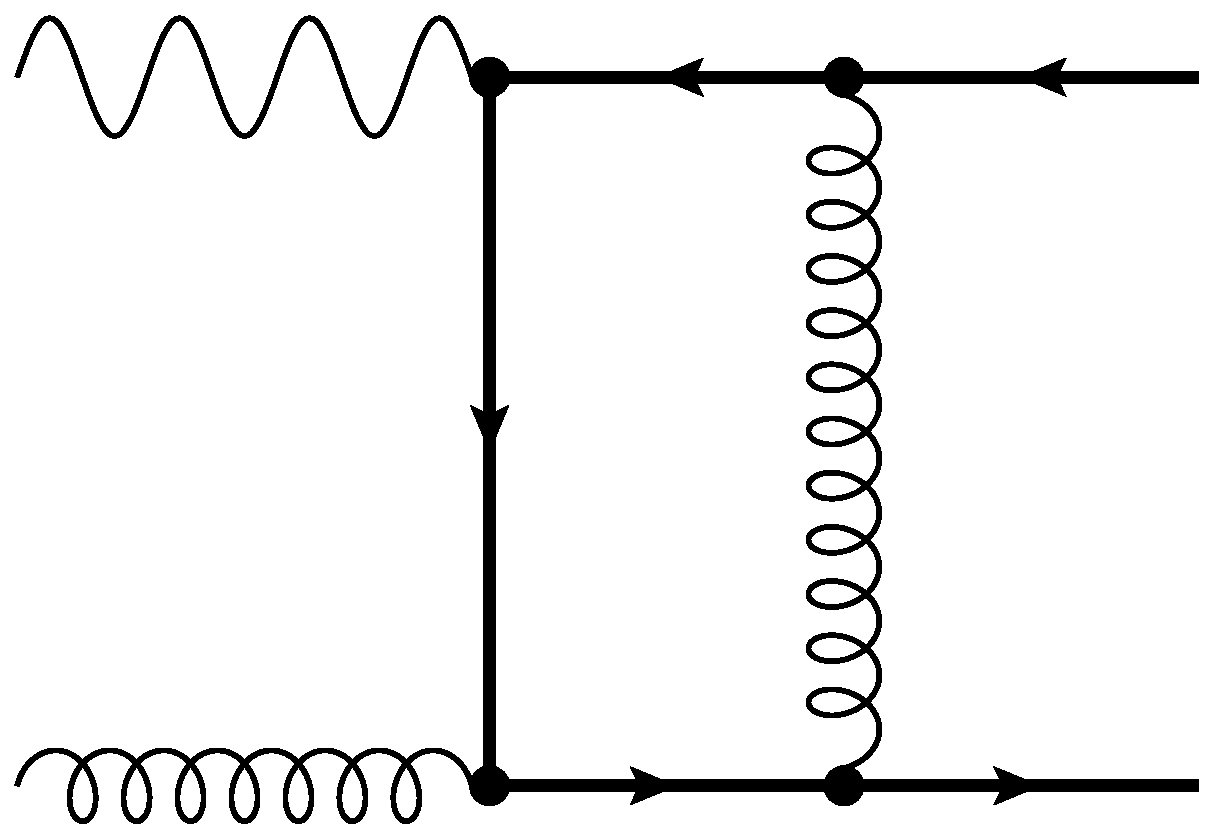
\includegraphics[width=.25\textwidth]{img/nlo-v-1}
&or
&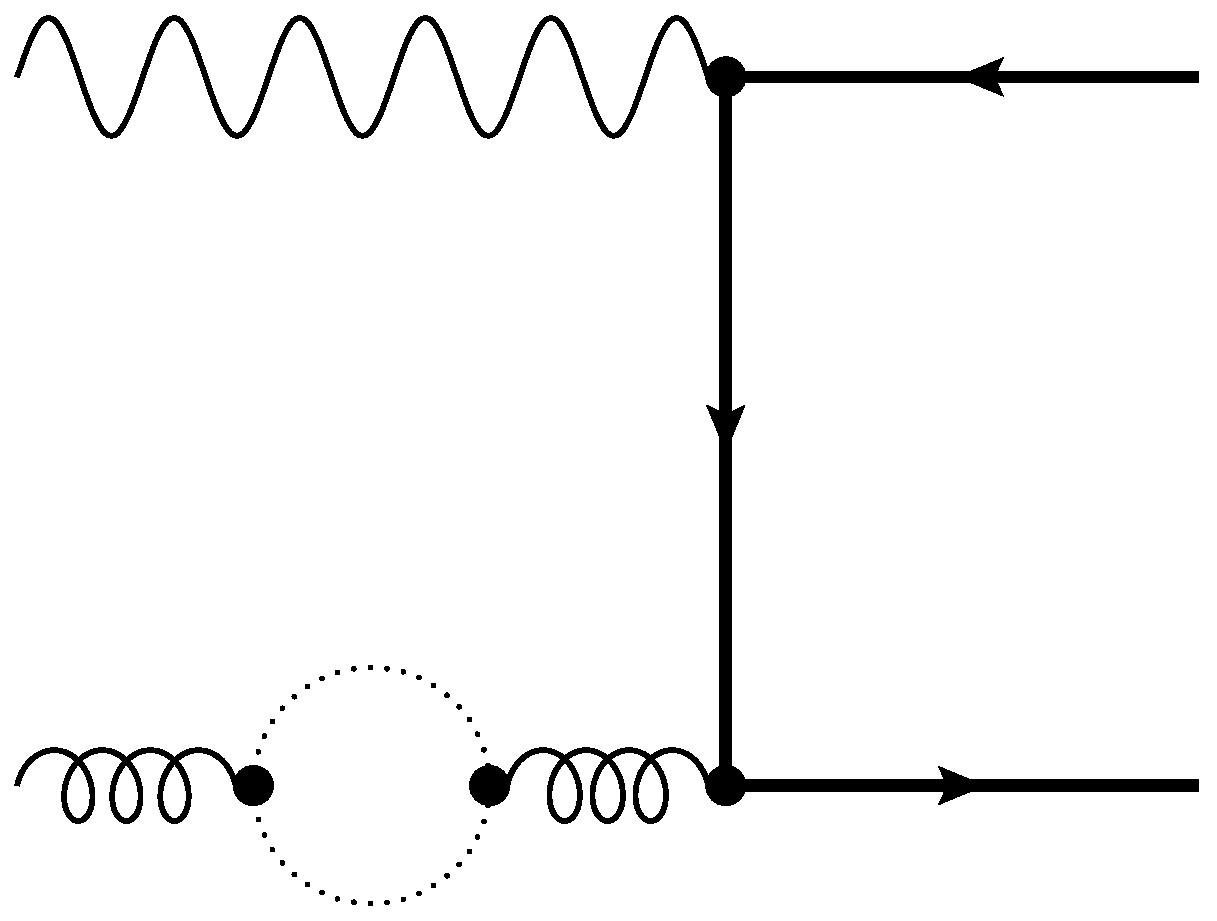
\includegraphics[width=.25\textwidth]{img/nlo-v-5}
\end{tabular}
\end{center}

soft poles appear in the limit of a soft gluon $k_2\rightarrow 0$, e.g.,
\begin{center}
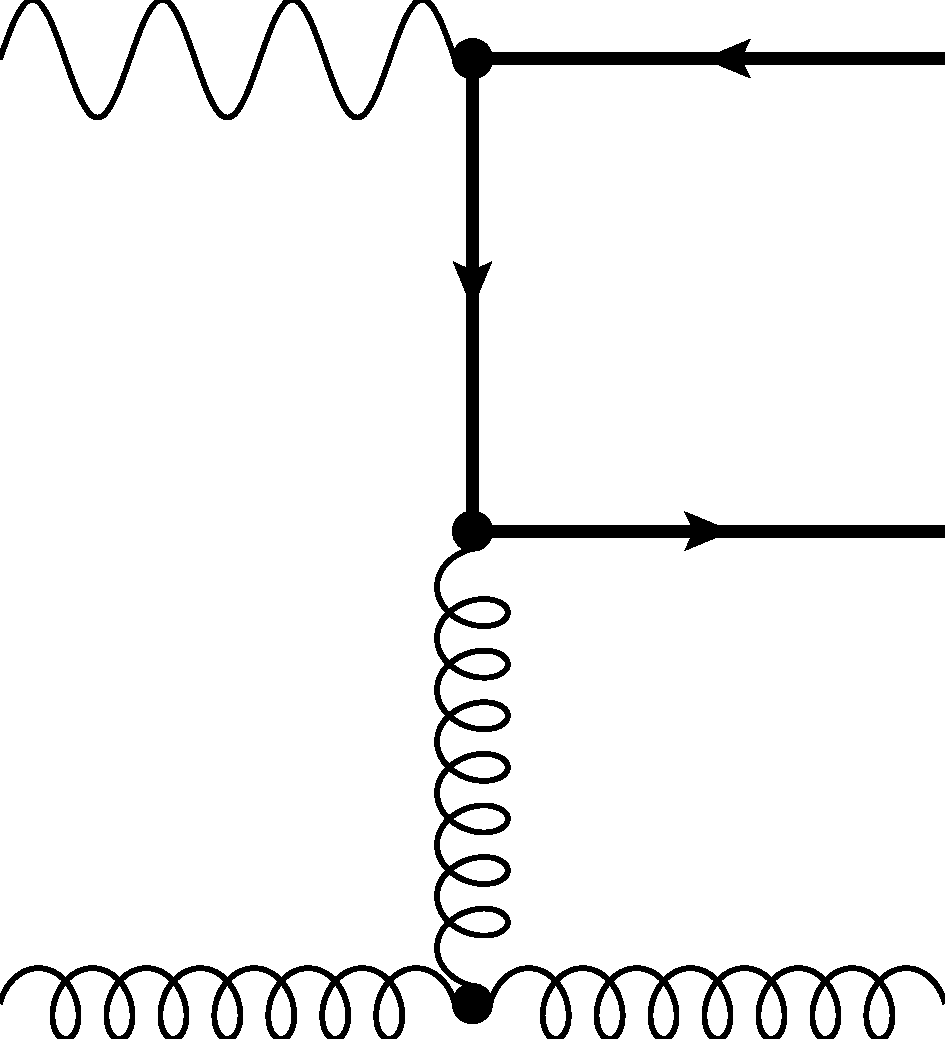
\includegraphics[width=.25\textwidth]{pyfeyn2/nlo-g-4}
\end{center}

soft + virtual + renormalization + factorization is finite!
\end{frame}


The \textit{total} partonic cross sections can be computed by
\begin{align}
\sigma^{(n)}_{k,j}(s,q^2,m^2) &= \int\limits_{-s'(1+\beta)/2}^{-s'(1-\beta)/2} dt_1\int\limits_0^{s_{4,max}}ds_4 \frac{d^2\sigma^{(n),fin}_{k,j}(s',t_1,u_1,q^2)}{dt_1ds_4}\\
s_{4,max} &= \frac{s}{s' t_1}\left(t_1+\frac{s'(1-\beta)}{2}\right)\left(t_1+\frac{s'(1+\beta)}{2}\right)
\end{align}
where $k$ denotes as usual projection, $j\in\{\Pg,\Pq,\Paq\}$ is a parton index and we used $s_4 = s'+t_1+u_1$. The result can then be parametrised as
\begin{align}
&\sigma_{k,j}(s,q^2,m^2)\nonumber\\
 &= \sigma^{(0)}_{k,j}(s,q^2,m^2) + \sigma^{(1)}_{k,j}(s,q^2,m^2)\\
 &= \frac{\alpha\alpha_S}{m^2}\left(f_{k,j}^{(0)}(\eta,\xi) + 4\pi\left(f_{k,j}^{(1)}(\eta,\xi) + \ln(\mu_F^2/m^2)\bar f_{k,j}^{F,(1)}(\eta,\xi) + \ln(\mu_R^2/m^2)\bar f_{k,j}^{R,(1)}(\eta,\xi)\right)\right)
\end{align}
where each function $f_{k,j}$ depends on the scaling variables $\eta=1/\rho-1$ and $\xi=-q^2/m^2$ and can be further decomposed by the electric charges
\begin{align}
f_{k,\Pg}(\eta,\xi) &= e_H^2 c_{k,\Pg}(\eta,\xi)\\
f_{k,\Pq}(\eta,\xi) &= e_H^2 c_{k,\Pq}(\eta,\xi) + e_L^2 d_{k,\Pq}(\eta,\xi)
\end{align}
As already mentioned the interference term proportional to $e_H e_L$ vanishes for total cross sections.

\fxerror{how to arrange 3 equal images? shift to appendix?}
\fxerror{compare T and P?}

\pagebreak
\begin{figure}[ht!]
\centering
\begin{subfigure}[t]{\textwidth}
	% GNUPLOT: LaTeX picture with Postscript
\begingroup
  \makeatletter
  \providecommand\color[2][]{%
    \GenericError{(gnuplot) \space\space\space\@spaces}{%
      Package color not loaded in conjunction with
      terminal option `colourtext'%
    }{See the gnuplot documentation for explanation.%
    }{Either use 'blacktext' in gnuplot or load the package
      color.sty in LaTeX.}%
    \renewcommand\color[2][]{}%
  }%
  \providecommand\includegraphics[2][]{%
    \GenericError{(gnuplot) \space\space\space\@spaces}{%
      Package graphicx or graphics not loaded%
    }{See the gnuplot documentation for explanation.%
    }{The gnuplot epslatex terminal needs graphicx.sty or graphics.sty.}%
    \renewcommand\includegraphics[2][]{}%
  }%
  \providecommand\rotatebox[2]{#2}%
  \@ifundefined{ifGPcolor}{%
    \newif\ifGPcolor
    \GPcolorfalse
  }{}%
  \@ifundefined{ifGPblacktext}{%
    \newif\ifGPblacktext
    \GPblacktexttrue
  }{}%
  % define a \g@addto@macro without @ in the name:
  \let\gplgaddtomacro\g@addto@macro
  % define empty templates for all commands taking text:
  \gdef\gplbacktext{}%
  \gdef\gplfronttext{}%
  \makeatother
  \ifGPblacktext
    % no textcolor at all
    \def\colorrgb#1{}%
    \def\colorgray#1{}%
  \else
    % gray or color?
    \ifGPcolor
      \def\colorrgb#1{\color[rgb]{#1}}%
      \def\colorgray#1{\color[gray]{#1}}%
      \expandafter\def\csname LTw\endcsname{\color{white}}%
      \expandafter\def\csname LTb\endcsname{\color{black}}%
      \expandafter\def\csname LTa\endcsname{\color{black}}%
      \expandafter\def\csname LT0\endcsname{\color[rgb]{1,0,0}}%
      \expandafter\def\csname LT1\endcsname{\color[rgb]{0,1,0}}%
      \expandafter\def\csname LT2\endcsname{\color[rgb]{0,0,1}}%
      \expandafter\def\csname LT3\endcsname{\color[rgb]{1,0,1}}%
      \expandafter\def\csname LT4\endcsname{\color[rgb]{0,1,1}}%
      \expandafter\def\csname LT5\endcsname{\color[rgb]{1,1,0}}%
      \expandafter\def\csname LT6\endcsname{\color[rgb]{0,0,0}}%
      \expandafter\def\csname LT7\endcsname{\color[rgb]{1,0.3,0}}%
      \expandafter\def\csname LT8\endcsname{\color[rgb]{0.5,0.5,0.5}}%
    \else
      % gray
      \def\colorrgb#1{\color{black}}%
      \def\colorgray#1{\color[gray]{#1}}%
      \expandafter\def\csname LTw\endcsname{\color{white}}%
      \expandafter\def\csname LTb\endcsname{\color{black}}%
      \expandafter\def\csname LTa\endcsname{\color{black}}%
      \expandafter\def\csname LT0\endcsname{\color{black}}%
      \expandafter\def\csname LT1\endcsname{\color{black}}%
      \expandafter\def\csname LT2\endcsname{\color{black}}%
      \expandafter\def\csname LT3\endcsname{\color{black}}%
      \expandafter\def\csname LT4\endcsname{\color{black}}%
      \expandafter\def\csname LT5\endcsname{\color{black}}%
      \expandafter\def\csname LT6\endcsname{\color{black}}%
      \expandafter\def\csname LT7\endcsname{\color{black}}%
      \expandafter\def\csname LT8\endcsname{\color{black}}%
    \fi
  \fi
    \setlength{\unitlength}{0.0500bp}%
    \ifx\gptboxheight\undefined%
      \newlength{\gptboxheight}%
      \newlength{\gptboxwidth}%
      \newsavebox{\gptboxtext}%
    \fi%
    \setlength{\fboxrule}{0.5pt}%
    \setlength{\fboxsep}{1pt}%
\begin{picture}(7920.00,4082.40)%
    \gplgaddtomacro\gplbacktext{%
      \csname LTb\endcsname%
      \put(726,220){\makebox(0,0)[r]{\strut{} 0.0}}%
      \put(726,820){\makebox(0,0)[r]{\strut{} 0.2}}%
      \put(726,1419){\makebox(0,0)[r]{\strut{} 0.4}}%
      \put(726,2019){\makebox(0,0)[r]{\strut{} 0.6}}%
      \put(726,2619){\makebox(0,0)[r]{\strut{} 0.8}}%
      \put(726,3218){\makebox(0,0)[r]{\strut{} 1.0}}%
      \put(726,3818){\makebox(0,0)[r]{\strut{} 1.2}}%
      \put(858,0){\makebox(0,0){\strut{}$0.001$}}%
      \put(1969,0){\makebox(0,0){\strut{}$0.01$}}%
      \put(3079,0){\makebox(0,0){\strut{}$0.1$}}%
      \put(4190,0){\makebox(0,0){\strut{}$1$}}%
      \put(5301,0){\makebox(0,0){\strut{}$10$}}%
      \put(6411,0){\makebox(0,0){\strut{}$100$}}%
      \put(7522,0){\makebox(0,0){\strut{}$1000$}}%
      \put(991,3458){\makebox(0,0)[l]{\strut{}(a) $c_{T,g}^{(0)}(\eta)$}}%
    }%
    \gplgaddtomacro\gplfronttext{%
      \csname LTb\endcsname%
      \put(5611,3645){\makebox(0,0)[l]{\strut{}$Q^2=10^{-2}$}}%
      \csname LTb\endcsname%
      \put(5611,3425){\makebox(0,0)[l]{\strut{}$Q^2=10^0$}}%
      \csname LTb\endcsname%
      \put(5611,3205){\makebox(0,0)[l]{\strut{}$Q^2=10^1$}}%
      \csname LTb\endcsname%
      \put(5611,2985){\makebox(0,0)[l]{\strut{}$Q^2=10^2$}}%
      \csname LTb\endcsname%
      \put(5611,2765){\makebox(0,0)[l]{\strut{}$Q^2=10^3$}}%
    }%
    \gplbacktext
    \put(0,0){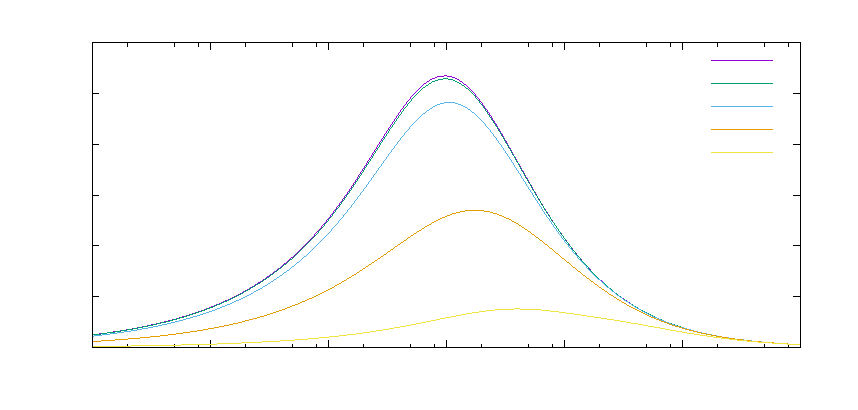
\includegraphics{img/cg0T}}%
    \gplfronttext
  \end{picture}%
\endgroup

	\caption{$c_{T,g}^{(0)}(\eta)$}
\end{subfigure}\\%
\begin{subfigure}[t]{\textwidth}
	% GNUPLOT: LaTeX picture with Postscript
\begingroup
  \makeatletter
  \providecommand\color[2][]{%
    \GenericError{(gnuplot) \space\space\space\@spaces}{%
      Package color not loaded in conjunction with
      terminal option `colourtext'%
    }{See the gnuplot documentation for explanation.%
    }{Either use 'blacktext' in gnuplot or load the package
      color.sty in LaTeX.}%
    \renewcommand\color[2][]{}%
  }%
  \providecommand\includegraphics[2][]{%
    \GenericError{(gnuplot) \space\space\space\@spaces}{%
      Package graphicx or graphics not loaded%
    }{See the gnuplot documentation for explanation.%
    }{The gnuplot epslatex terminal needs graphicx.sty or graphics.sty.}%
    \renewcommand\includegraphics[2][]{}%
  }%
  \providecommand\rotatebox[2]{#2}%
  \@ifundefined{ifGPcolor}{%
    \newif\ifGPcolor
    \GPcolorfalse
  }{}%
  \@ifundefined{ifGPblacktext}{%
    \newif\ifGPblacktext
    \GPblacktexttrue
  }{}%
  % define a \g@addto@macro without @ in the name:
  \let\gplgaddtomacro\g@addto@macro
  % define empty templates for all commands taking text:
  \gdef\gplbacktext{}%
  \gdef\gplfronttext{}%
  \makeatother
  \ifGPblacktext
    % no textcolor at all
    \def\colorrgb#1{}%
    \def\colorgray#1{}%
  \else
    % gray or color?
    \ifGPcolor
      \def\colorrgb#1{\color[rgb]{#1}}%
      \def\colorgray#1{\color[gray]{#1}}%
      \expandafter\def\csname LTw\endcsname{\color{white}}%
      \expandafter\def\csname LTb\endcsname{\color{black}}%
      \expandafter\def\csname LTa\endcsname{\color{black}}%
      \expandafter\def\csname LT0\endcsname{\color[rgb]{1,0,0}}%
      \expandafter\def\csname LT1\endcsname{\color[rgb]{0,1,0}}%
      \expandafter\def\csname LT2\endcsname{\color[rgb]{0,0,1}}%
      \expandafter\def\csname LT3\endcsname{\color[rgb]{1,0,1}}%
      \expandafter\def\csname LT4\endcsname{\color[rgb]{0,1,1}}%
      \expandafter\def\csname LT5\endcsname{\color[rgb]{1,1,0}}%
      \expandafter\def\csname LT6\endcsname{\color[rgb]{0,0,0}}%
      \expandafter\def\csname LT7\endcsname{\color[rgb]{1,0.3,0}}%
      \expandafter\def\csname LT8\endcsname{\color[rgb]{0.5,0.5,0.5}}%
    \else
      % gray
      \def\colorrgb#1{\color{black}}%
      \def\colorgray#1{\color[gray]{#1}}%
      \expandafter\def\csname LTw\endcsname{\color{white}}%
      \expandafter\def\csname LTb\endcsname{\color{black}}%
      \expandafter\def\csname LTa\endcsname{\color{black}}%
      \expandafter\def\csname LT0\endcsname{\color{black}}%
      \expandafter\def\csname LT1\endcsname{\color{black}}%
      \expandafter\def\csname LT2\endcsname{\color{black}}%
      \expandafter\def\csname LT3\endcsname{\color{black}}%
      \expandafter\def\csname LT4\endcsname{\color{black}}%
      \expandafter\def\csname LT5\endcsname{\color{black}}%
      \expandafter\def\csname LT6\endcsname{\color{black}}%
      \expandafter\def\csname LT7\endcsname{\color{black}}%
      \expandafter\def\csname LT8\endcsname{\color{black}}%
    \fi
  \fi
    \setlength{\unitlength}{0.0500bp}%
    \ifx\gptboxheight\undefined%
      \newlength{\gptboxheight}%
      \newlength{\gptboxwidth}%
      \newsavebox{\gptboxtext}%
    \fi%
    \setlength{\fboxrule}{0.5pt}%
    \setlength{\fboxsep}{1pt}%
\begin{picture}(7920.00,4082.40)%
    \gplgaddtomacro\gplbacktext{%
      \csname LTb\endcsname%
      \put(726,220){\makebox(0,0)[r]{\strut{}0.00}}%
      \put(726,734){\makebox(0,0)[r]{\strut{}0.02}}%
      \put(726,1248){\makebox(0,0)[r]{\strut{}0.04}}%
      \put(726,1762){\makebox(0,0)[r]{\strut{}0.06}}%
      \put(726,2276){\makebox(0,0)[r]{\strut{}0.08}}%
      \put(726,2790){\makebox(0,0)[r]{\strut{}0.10}}%
      \put(726,3304){\makebox(0,0)[r]{\strut{}0.12}}%
      \put(726,3818){\makebox(0,0)[r]{\strut{}0.14}}%
      \put(858,0){\makebox(0,0){\strut{}$0.001$}}%
      \put(1969,0){\makebox(0,0){\strut{}$0.01$}}%
      \put(3079,0){\makebox(0,0){\strut{}$0.1$}}%
      \put(4190,0){\makebox(0,0){\strut{}$1$}}%
      \put(5301,0){\makebox(0,0){\strut{}$10$}}%
      \put(6411,0){\makebox(0,0){\strut{}$100$}}%
      \put(7522,0){\makebox(0,0){\strut{}$1000$}}%
      \put(991,3458){\makebox(0,0)[l]{\strut{}(b) $c_{L,g}^{(0)}(\eta)$}}%
    }%
    \gplgaddtomacro\gplfronttext{%
      \csname LTb\endcsname%
      \put(5611,3645){\makebox(0,0)[l]{\strut{}$Q^2=10^{-2}$}}%
      \csname LTb\endcsname%
      \put(5611,3425){\makebox(0,0)[l]{\strut{}$Q^2=10^0$}}%
      \csname LTb\endcsname%
      \put(5611,3205){\makebox(0,0)[l]{\strut{}$Q^2=10^1$}}%
      \csname LTb\endcsname%
      \put(5611,2985){\makebox(0,0)[l]{\strut{}$Q^2=10^2$}}%
      \csname LTb\endcsname%
      \put(5611,2765){\makebox(0,0)[l]{\strut{}$Q^2=10^3$}}%
    }%
    \gplbacktext
    \put(0,0){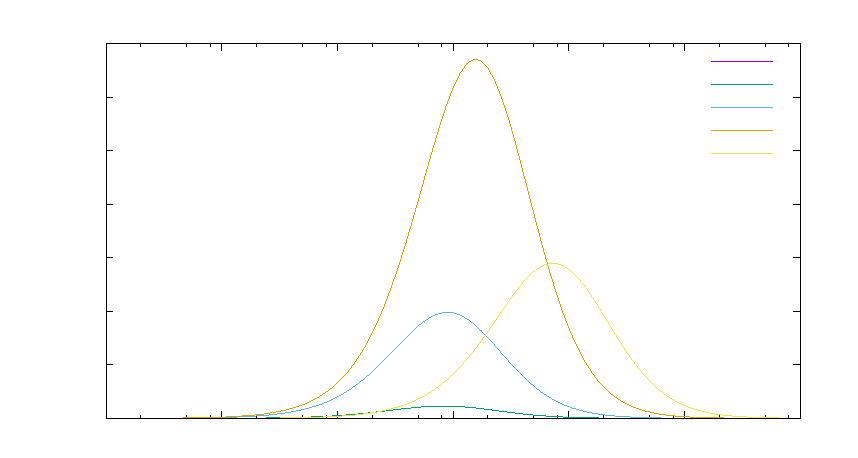
\includegraphics{img/cg0L}}%
    \gplfronttext
  \end{picture}%
\endgroup

	\caption{$c_{L,g}^{(0)}(\eta)$}
\end{subfigure}\\%
\begin{subfigure}[t]{\textwidth}
	% GNUPLOT: LaTeX picture with Postscript
\begingroup
  \makeatletter
  \providecommand\color[2][]{%
    \GenericError{(gnuplot) \space\space\space\@spaces}{%
      Package color not loaded in conjunction with
      terminal option `colourtext'%
    }{See the gnuplot documentation for explanation.%
    }{Either use 'blacktext' in gnuplot or load the package
      color.sty in LaTeX.}%
    \renewcommand\color[2][]{}%
  }%
  \providecommand\includegraphics[2][]{%
    \GenericError{(gnuplot) \space\space\space\@spaces}{%
      Package graphicx or graphics not loaded%
    }{See the gnuplot documentation for explanation.%
    }{The gnuplot epslatex terminal needs graphicx.sty or graphics.sty.}%
    \renewcommand\includegraphics[2][]{}%
  }%
  \providecommand\rotatebox[2]{#2}%
  \@ifundefined{ifGPcolor}{%
    \newif\ifGPcolor
    \GPcolorfalse
  }{}%
  \@ifundefined{ifGPblacktext}{%
    \newif\ifGPblacktext
    \GPblacktexttrue
  }{}%
  % define a \g@addto@macro without @ in the name:
  \let\gplgaddtomacro\g@addto@macro
  % define empty templates for all commands taking text:
  \gdef\gplbacktext{}%
  \gdef\gplfronttext{}%
  \makeatother
  \ifGPblacktext
    % no textcolor at all
    \def\colorrgb#1{}%
    \def\colorgray#1{}%
  \else
    % gray or color?
    \ifGPcolor
      \def\colorrgb#1{\color[rgb]{#1}}%
      \def\colorgray#1{\color[gray]{#1}}%
      \expandafter\def\csname LTw\endcsname{\color{white}}%
      \expandafter\def\csname LTb\endcsname{\color{black}}%
      \expandafter\def\csname LTa\endcsname{\color{black}}%
      \expandafter\def\csname LT0\endcsname{\color[rgb]{1,0,0}}%
      \expandafter\def\csname LT1\endcsname{\color[rgb]{0,1,0}}%
      \expandafter\def\csname LT2\endcsname{\color[rgb]{0,0,1}}%
      \expandafter\def\csname LT3\endcsname{\color[rgb]{1,0,1}}%
      \expandafter\def\csname LT4\endcsname{\color[rgb]{0,1,1}}%
      \expandafter\def\csname LT5\endcsname{\color[rgb]{1,1,0}}%
      \expandafter\def\csname LT6\endcsname{\color[rgb]{0,0,0}}%
      \expandafter\def\csname LT7\endcsname{\color[rgb]{1,0.3,0}}%
      \expandafter\def\csname LT8\endcsname{\color[rgb]{0.5,0.5,0.5}}%
    \else
      % gray
      \def\colorrgb#1{\color{black}}%
      \def\colorgray#1{\color[gray]{#1}}%
      \expandafter\def\csname LTw\endcsname{\color{white}}%
      \expandafter\def\csname LTb\endcsname{\color{black}}%
      \expandafter\def\csname LTa\endcsname{\color{black}}%
      \expandafter\def\csname LT0\endcsname{\color{black}}%
      \expandafter\def\csname LT1\endcsname{\color{black}}%
      \expandafter\def\csname LT2\endcsname{\color{black}}%
      \expandafter\def\csname LT3\endcsname{\color{black}}%
      \expandafter\def\csname LT4\endcsname{\color{black}}%
      \expandafter\def\csname LT5\endcsname{\color{black}}%
      \expandafter\def\csname LT6\endcsname{\color{black}}%
      \expandafter\def\csname LT7\endcsname{\color{black}}%
      \expandafter\def\csname LT8\endcsname{\color{black}}%
    \fi
  \fi
    \setlength{\unitlength}{0.0500bp}%
    \ifx\gptboxheight\undefined%
      \newlength{\gptboxheight}%
      \newlength{\gptboxwidth}%
      \newsavebox{\gptboxtext}%
    \fi%
    \setlength{\fboxrule}{0.5pt}%
    \setlength{\fboxsep}{1pt}%
\begin{picture}(7920.00,4082.40)%
    \gplgaddtomacro\gplbacktext{%
      \csname LTb\endcsname%
      \put(726,220){\makebox(0,0)[r]{\strut{}-0.2}}%
      \put(726,734){\makebox(0,0)[r]{\strut{}-0.1}}%
      \put(726,1248){\makebox(0,0)[r]{\strut{}0.0}}%
      \put(726,1762){\makebox(0,0)[r]{\strut{}0.1}}%
      \put(726,2276){\makebox(0,0)[r]{\strut{}0.2}}%
      \put(726,2790){\makebox(0,0)[r]{\strut{}0.3}}%
      \put(726,3304){\makebox(0,0)[r]{\strut{}0.4}}%
      \put(726,3818){\makebox(0,0)[r]{\strut{}0.5}}%
      \put(858,0){\makebox(0,0){\strut{}$0.001$}}%
      \put(1969,0){\makebox(0,0){\strut{}$0.01$}}%
      \put(3079,0){\makebox(0,0){\strut{}$0.1$}}%
      \put(4190,0){\makebox(0,0){\strut{}$1$}}%
      \put(5301,0){\makebox(0,0){\strut{}$10$}}%
      \put(6411,0){\makebox(0,0){\strut{}$100$}}%
      \put(7522,0){\makebox(0,0){\strut{}$1000$}}%
      \put(991,3458){\makebox(0,0)[l]{\strut{}(c) $c_{P,g}^{(0)}(\eta)$}}%
    }%
    \gplgaddtomacro\gplfronttext{%
      \csname LTb\endcsname%
      \put(5611,3645){\makebox(0,0)[l]{\strut{}$Q^2=10^{-2}$}}%
      \csname LTb\endcsname%
      \put(5611,3425){\makebox(0,0)[l]{\strut{}$Q^2=10^0$}}%
      \csname LTb\endcsname%
      \put(5611,3205){\makebox(0,0)[l]{\strut{}$Q^2=10^1$}}%
      \csname LTb\endcsname%
      \put(5611,2985){\makebox(0,0)[l]{\strut{}$Q^2=10^2$}}%
      \csname LTb\endcsname%
      \put(5611,2765){\makebox(0,0)[l]{\strut{}$Q^2=10^3$}}%
    }%
    \gplbacktext
    \put(0,0){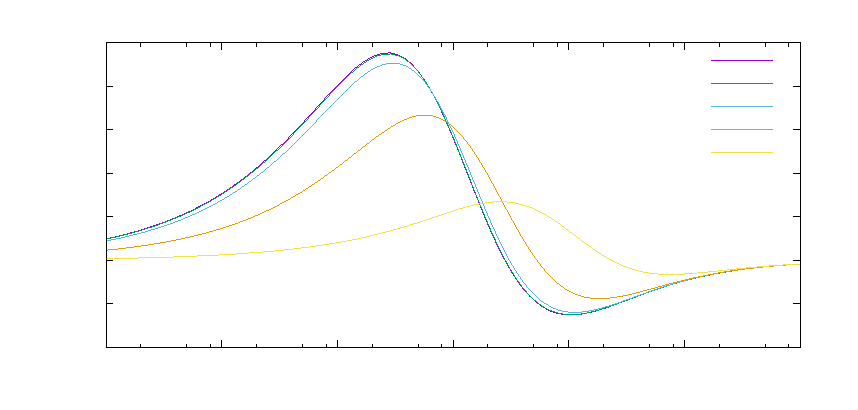
\includegraphics{img/cg0P}}%
    \gplfronttext
  \end{picture}%
\endgroup

	\caption{$c_{P,g}^{(0)}(\eta)$}
\end{subfigure}
\caption{leading order scaling functions $c_{k,g}^{(0)}(\eta,\xi)$ plotted as function of $\eta=s/(4m^2)-1$ for different values of $Q^2$ in units of $\si{\GeV^2}$ at $m=\SI{4.75}{\GeV}$ (i.e. different values of $\xi=Q^2/m^2$) }\label{fig:cg0}
\end{figure}

\pagebreak
\begin{figure}[ht!]
\centering
\begin{subfigure}[t]{\textwidth}
	% GNUPLOT: LaTeX picture with Postscript
\begingroup
  \makeatletter
  \providecommand\color[2][]{%
    \GenericError{(gnuplot) \space\space\space\@spaces}{%
      Package color not loaded in conjunction with
      terminal option `colourtext'%
    }{See the gnuplot documentation for explanation.%
    }{Either use 'blacktext' in gnuplot or load the package
      color.sty in LaTeX.}%
    \renewcommand\color[2][]{}%
  }%
  \providecommand\includegraphics[2][]{%
    \GenericError{(gnuplot) \space\space\space\@spaces}{%
      Package graphicx or graphics not loaded%
    }{See the gnuplot documentation for explanation.%
    }{The gnuplot epslatex terminal needs graphicx.sty or graphics.sty.}%
    \renewcommand\includegraphics[2][]{}%
  }%
  \providecommand\rotatebox[2]{#2}%
  \@ifundefined{ifGPcolor}{%
    \newif\ifGPcolor
    \GPcolorfalse
  }{}%
  \@ifundefined{ifGPblacktext}{%
    \newif\ifGPblacktext
    \GPblacktexttrue
  }{}%
  % define a \g@addto@macro without @ in the name:
  \let\gplgaddtomacro\g@addto@macro
  % define empty templates for all commands taking text:
  \gdef\gplbacktext{}%
  \gdef\gplfronttext{}%
  \makeatother
  \ifGPblacktext
    % no textcolor at all
    \def\colorrgb#1{}%
    \def\colorgray#1{}%
  \else
    % gray or color?
    \ifGPcolor
      \def\colorrgb#1{\color[rgb]{#1}}%
      \def\colorgray#1{\color[gray]{#1}}%
      \expandafter\def\csname LTw\endcsname{\color{white}}%
      \expandafter\def\csname LTb\endcsname{\color{black}}%
      \expandafter\def\csname LTa\endcsname{\color{black}}%
      \expandafter\def\csname LT0\endcsname{\color[rgb]{1,0,0}}%
      \expandafter\def\csname LT1\endcsname{\color[rgb]{0,1,0}}%
      \expandafter\def\csname LT2\endcsname{\color[rgb]{0,0,1}}%
      \expandafter\def\csname LT3\endcsname{\color[rgb]{1,0,1}}%
      \expandafter\def\csname LT4\endcsname{\color[rgb]{0,1,1}}%
      \expandafter\def\csname LT5\endcsname{\color[rgb]{1,1,0}}%
      \expandafter\def\csname LT6\endcsname{\color[rgb]{0,0,0}}%
      \expandafter\def\csname LT7\endcsname{\color[rgb]{1,0.3,0}}%
      \expandafter\def\csname LT8\endcsname{\color[rgb]{0.5,0.5,0.5}}%
    \else
      % gray
      \def\colorrgb#1{\color{black}}%
      \def\colorgray#1{\color[gray]{#1}}%
      \expandafter\def\csname LTw\endcsname{\color{white}}%
      \expandafter\def\csname LTb\endcsname{\color{black}}%
      \expandafter\def\csname LTa\endcsname{\color{black}}%
      \expandafter\def\csname LT0\endcsname{\color{black}}%
      \expandafter\def\csname LT1\endcsname{\color{black}}%
      \expandafter\def\csname LT2\endcsname{\color{black}}%
      \expandafter\def\csname LT3\endcsname{\color{black}}%
      \expandafter\def\csname LT4\endcsname{\color{black}}%
      \expandafter\def\csname LT5\endcsname{\color{black}}%
      \expandafter\def\csname LT6\endcsname{\color{black}}%
      \expandafter\def\csname LT7\endcsname{\color{black}}%
      \expandafter\def\csname LT8\endcsname{\color{black}}%
    \fi
  \fi
    \setlength{\unitlength}{0.0500bp}%
    \ifx\gptboxheight\undefined%
      \newlength{\gptboxheight}%
      \newlength{\gptboxwidth}%
      \newsavebox{\gptboxtext}%
    \fi%
    \setlength{\fboxrule}{0.5pt}%
    \setlength{\fboxsep}{1pt}%
\begin{picture}(7920.00,3628.80)%
    \gplgaddtomacro\gplbacktext{%
      \csname LTb\endcsname%
      \put(726,440){\makebox(0,0)[r]{\strut{}-0.1}}%
      \put(726,806){\makebox(0,0)[r]{\strut{}0.0}}%
      \put(726,1171){\makebox(0,0)[r]{\strut{}0.1}}%
      \put(726,1537){\makebox(0,0)[r]{\strut{}0.1}}%
      \put(726,1902){\makebox(0,0)[r]{\strut{}0.2}}%
      \put(726,2268){\makebox(0,0)[r]{\strut{}0.2}}%
      \put(726,2633){\makebox(0,0)[r]{\strut{}0.2}}%
      \put(726,2999){\makebox(0,0)[r]{\strut{}0.3}}%
      \put(726,3364){\makebox(0,0)[r]{\strut{}0.3}}%
      \put(858,220){\makebox(0,0){\strut{}$0.001$}}%
      \put(1969,220){\makebox(0,0){\strut{}$0.01$}}%
      \put(3079,220){\makebox(0,0){\strut{}$0.1$}}%
      \put(4190,220){\makebox(0,0){\strut{}$1$}}%
      \put(5301,220){\makebox(0,0){\strut{}$10$}}%
      \put(6411,220){\makebox(0,0){\strut{}$100$}}%
      \put(7522,220){\makebox(0,0){\strut{}$1000$}}%
    }%
    \gplgaddtomacro\gplfronttext{%
      \csname LTb\endcsname%
      \put(4077,3108){\makebox(0,0)[l]{\strut{}$Q^2=10^{-2}$}}%
      \csname LTb\endcsname%
      \put(4077,2888){\makebox(0,0)[l]{\strut{}$Q^2=10^0$}}%
      \csname LTb\endcsname%
      \put(4077,2668){\makebox(0,0)[l]{\strut{}$Q^2=10^1$}}%
      \csname LTb\endcsname%
      \put(4077,2448){\makebox(0,0)[l]{\strut{}$Q^2=10^2$}}%
      \csname LTb\endcsname%
      \put(4077,2228){\makebox(0,0)[l]{\strut{}$Q^2=10^3$}}%
    }%
    \gplbacktext
    \put(0,0){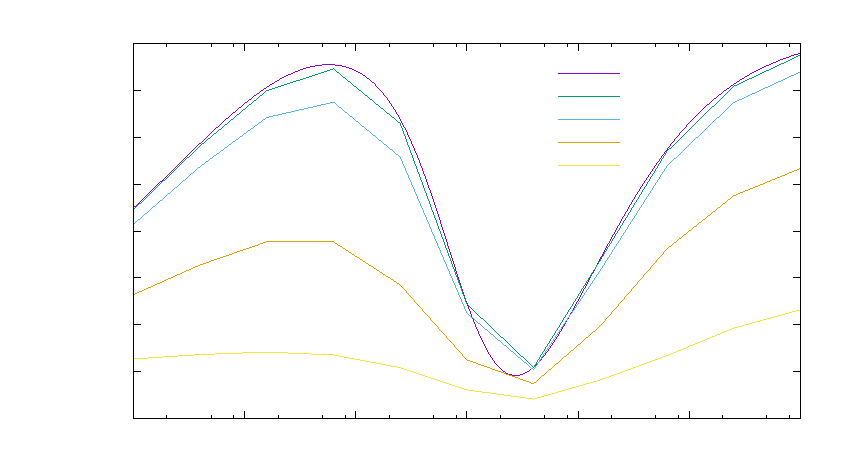
\includegraphics{img/cg1T}}%
    \gplfronttext
  \end{picture}%
\endgroup

	\caption{$c_{T,g}^{(1)}(\eta)$}
\end{subfigure}\\%
\begin{subfigure}[t]{\textwidth}
	% GNUPLOT: LaTeX picture with Postscript
\begingroup
  \makeatletter
  \providecommand\color[2][]{%
    \GenericError{(gnuplot) \space\space\space\@spaces}{%
      Package color not loaded in conjunction with
      terminal option `colourtext'%
    }{See the gnuplot documentation for explanation.%
    }{Either use 'blacktext' in gnuplot or load the package
      color.sty in LaTeX.}%
    \renewcommand\color[2][]{}%
  }%
  \providecommand\includegraphics[2][]{%
    \GenericError{(gnuplot) \space\space\space\@spaces}{%
      Package graphicx or graphics not loaded%
    }{See the gnuplot documentation for explanation.%
    }{The gnuplot epslatex terminal needs graphicx.sty or graphics.sty.}%
    \renewcommand\includegraphics[2][]{}%
  }%
  \providecommand\rotatebox[2]{#2}%
  \@ifundefined{ifGPcolor}{%
    \newif\ifGPcolor
    \GPcolorfalse
  }{}%
  \@ifundefined{ifGPblacktext}{%
    \newif\ifGPblacktext
    \GPblacktexttrue
  }{}%
  % define a \g@addto@macro without @ in the name:
  \let\gplgaddtomacro\g@addto@macro
  % define empty templates for all commands taking text:
  \gdef\gplbacktext{}%
  \gdef\gplfronttext{}%
  \makeatother
  \ifGPblacktext
    % no textcolor at all
    \def\colorrgb#1{}%
    \def\colorgray#1{}%
  \else
    % gray or color?
    \ifGPcolor
      \def\colorrgb#1{\color[rgb]{#1}}%
      \def\colorgray#1{\color[gray]{#1}}%
      \expandafter\def\csname LTw\endcsname{\color{white}}%
      \expandafter\def\csname LTb\endcsname{\color{black}}%
      \expandafter\def\csname LTa\endcsname{\color{black}}%
      \expandafter\def\csname LT0\endcsname{\color[rgb]{1,0,0}}%
      \expandafter\def\csname LT1\endcsname{\color[rgb]{0,1,0}}%
      \expandafter\def\csname LT2\endcsname{\color[rgb]{0,0,1}}%
      \expandafter\def\csname LT3\endcsname{\color[rgb]{1,0,1}}%
      \expandafter\def\csname LT4\endcsname{\color[rgb]{0,1,1}}%
      \expandafter\def\csname LT5\endcsname{\color[rgb]{1,1,0}}%
      \expandafter\def\csname LT6\endcsname{\color[rgb]{0,0,0}}%
      \expandafter\def\csname LT7\endcsname{\color[rgb]{1,0.3,0}}%
      \expandafter\def\csname LT8\endcsname{\color[rgb]{0.5,0.5,0.5}}%
    \else
      % gray
      \def\colorrgb#1{\color{black}}%
      \def\colorgray#1{\color[gray]{#1}}%
      \expandafter\def\csname LTw\endcsname{\color{white}}%
      \expandafter\def\csname LTb\endcsname{\color{black}}%
      \expandafter\def\csname LTa\endcsname{\color{black}}%
      \expandafter\def\csname LT0\endcsname{\color{black}}%
      \expandafter\def\csname LT1\endcsname{\color{black}}%
      \expandafter\def\csname LT2\endcsname{\color{black}}%
      \expandafter\def\csname LT3\endcsname{\color{black}}%
      \expandafter\def\csname LT4\endcsname{\color{black}}%
      \expandafter\def\csname LT5\endcsname{\color{black}}%
      \expandafter\def\csname LT6\endcsname{\color{black}}%
      \expandafter\def\csname LT7\endcsname{\color{black}}%
      \expandafter\def\csname LT8\endcsname{\color{black}}%
    \fi
  \fi
    \setlength{\unitlength}{0.0500bp}%
    \ifx\gptboxheight\undefined%
      \newlength{\gptboxheight}%
      \newlength{\gptboxwidth}%
      \newsavebox{\gptboxtext}%
    \fi%
    \setlength{\fboxrule}{0.5pt}%
    \setlength{\fboxsep}{1pt}%
\begin{picture}(7920.00,4082.40)%
    \gplgaddtomacro\gplbacktext{%
      \csname LTb\endcsname%
      \put(990,220){\makebox(0,0)[r]{\strut{}-0.015}}%
      \put(990,620){\makebox(0,0)[r]{\strut{}-0.010}}%
      \put(990,1020){\makebox(0,0)[r]{\strut{}-0.005}}%
      \put(990,1419){\makebox(0,0)[r]{\strut{}0.000}}%
      \put(990,1819){\makebox(0,0)[r]{\strut{}0.005}}%
      \put(990,2219){\makebox(0,0)[r]{\strut{}0.010}}%
      \put(990,2619){\makebox(0,0)[r]{\strut{}0.015}}%
      \put(990,3018){\makebox(0,0)[r]{\strut{}0.020}}%
      \put(990,3418){\makebox(0,0)[r]{\strut{}0.025}}%
      \put(990,3818){\makebox(0,0)[r]{\strut{}0.030}}%
      \put(1122,0){\makebox(0,0){\strut{}$0.001$}}%
      \put(2189,0){\makebox(0,0){\strut{}$0.01$}}%
      \put(3255,0){\makebox(0,0){\strut{}$0.1$}}%
      \put(4322,0){\makebox(0,0){\strut{}$1$}}%
      \put(5389,0){\makebox(0,0){\strut{}$10$}}%
      \put(6455,0){\makebox(0,0){\strut{}$100$}}%
      \put(7522,0){\makebox(0,0){\strut{}$1000$}}%
      \put(1250,472){\makebox(0,0)[l]{\strut{}(b) $c_{L,g}^{(1)}(\eta)$}}%
    }%
    \gplgaddtomacro\gplfronttext{%
      \csname LTb\endcsname%
      \put(1254,3645){\makebox(0,0)[l]{\strut{}$Q^2=10^{-2}$}}%
      \csname LTb\endcsname%
      \put(1254,3425){\makebox(0,0)[l]{\strut{}$Q^2=10^0$}}%
      \csname LTb\endcsname%
      \put(1254,3205){\makebox(0,0)[l]{\strut{}$Q^2=10^1$}}%
      \csname LTb\endcsname%
      \put(1254,2985){\makebox(0,0)[l]{\strut{}$Q^2=10^2$}}%
      \csname LTb\endcsname%
      \put(1254,2765){\makebox(0,0)[l]{\strut{}$Q^2=10^3$}}%
    }%
    \gplbacktext
    \put(0,0){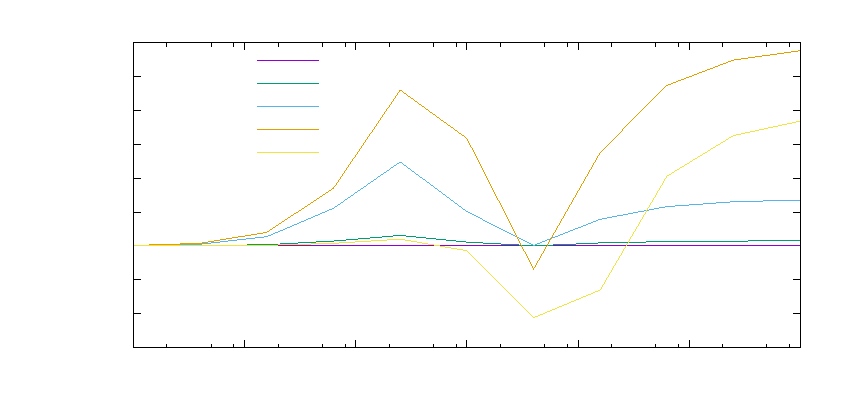
\includegraphics{img/cg1L}}%
    \gplfronttext
  \end{picture}%
\endgroup

	\caption{$c_{L,g}^{(1)}(\eta)$}
\end{subfigure}\\%
\begin{subfigure}[t]{\textwidth}
	% GNUPLOT: LaTeX picture with Postscript
\begingroup
  \makeatletter
  \providecommand\color[2][]{%
    \GenericError{(gnuplot) \space\space\space\@spaces}{%
      Package color not loaded in conjunction with
      terminal option `colourtext'%
    }{See the gnuplot documentation for explanation.%
    }{Either use 'blacktext' in gnuplot or load the package
      color.sty in LaTeX.}%
    \renewcommand\color[2][]{}%
  }%
  \providecommand\includegraphics[2][]{%
    \GenericError{(gnuplot) \space\space\space\@spaces}{%
      Package graphicx or graphics not loaded%
    }{See the gnuplot documentation for explanation.%
    }{The gnuplot epslatex terminal needs graphicx.sty or graphics.sty.}%
    \renewcommand\includegraphics[2][]{}%
  }%
  \providecommand\rotatebox[2]{#2}%
  \@ifundefined{ifGPcolor}{%
    \newif\ifGPcolor
    \GPcolorfalse
  }{}%
  \@ifundefined{ifGPblacktext}{%
    \newif\ifGPblacktext
    \GPblacktexttrue
  }{}%
  % define a \g@addto@macro without @ in the name:
  \let\gplgaddtomacro\g@addto@macro
  % define empty templates for all commands taking text:
  \gdef\gplbacktext{}%
  \gdef\gplfronttext{}%
  \makeatother
  \ifGPblacktext
    % no textcolor at all
    \def\colorrgb#1{}%
    \def\colorgray#1{}%
  \else
    % gray or color?
    \ifGPcolor
      \def\colorrgb#1{\color[rgb]{#1}}%
      \def\colorgray#1{\color[gray]{#1}}%
      \expandafter\def\csname LTw\endcsname{\color{white}}%
      \expandafter\def\csname LTb\endcsname{\color{black}}%
      \expandafter\def\csname LTa\endcsname{\color{black}}%
      \expandafter\def\csname LT0\endcsname{\color[rgb]{1,0,0}}%
      \expandafter\def\csname LT1\endcsname{\color[rgb]{0,1,0}}%
      \expandafter\def\csname LT2\endcsname{\color[rgb]{0,0,1}}%
      \expandafter\def\csname LT3\endcsname{\color[rgb]{1,0,1}}%
      \expandafter\def\csname LT4\endcsname{\color[rgb]{0,1,1}}%
      \expandafter\def\csname LT5\endcsname{\color[rgb]{1,1,0}}%
      \expandafter\def\csname LT6\endcsname{\color[rgb]{0,0,0}}%
      \expandafter\def\csname LT7\endcsname{\color[rgb]{1,0.3,0}}%
      \expandafter\def\csname LT8\endcsname{\color[rgb]{0.5,0.5,0.5}}%
    \else
      % gray
      \def\colorrgb#1{\color{black}}%
      \def\colorgray#1{\color[gray]{#1}}%
      \expandafter\def\csname LTw\endcsname{\color{white}}%
      \expandafter\def\csname LTb\endcsname{\color{black}}%
      \expandafter\def\csname LTa\endcsname{\color{black}}%
      \expandafter\def\csname LT0\endcsname{\color{black}}%
      \expandafter\def\csname LT1\endcsname{\color{black}}%
      \expandafter\def\csname LT2\endcsname{\color{black}}%
      \expandafter\def\csname LT3\endcsname{\color{black}}%
      \expandafter\def\csname LT4\endcsname{\color{black}}%
      \expandafter\def\csname LT5\endcsname{\color{black}}%
      \expandafter\def\csname LT6\endcsname{\color{black}}%
      \expandafter\def\csname LT7\endcsname{\color{black}}%
      \expandafter\def\csname LT8\endcsname{\color{black}}%
    \fi
  \fi
    \setlength{\unitlength}{0.0500bp}%
    \ifx\gptboxheight\undefined%
      \newlength{\gptboxheight}%
      \newlength{\gptboxwidth}%
      \newsavebox{\gptboxtext}%
    \fi%
    \setlength{\fboxrule}{0.5pt}%
    \setlength{\fboxsep}{1pt}%
\begin{picture}(7920.00,3628.80)%
    \gplgaddtomacro\gplbacktext{%
      \csname LTb\endcsname%
      \put(726,440){\makebox(0,0)[r]{\strut{}-0.2}}%
      \put(726,765){\makebox(0,0)[r]{\strut{}-0.1}}%
      \put(726,1090){\makebox(0,0)[r]{\strut{}-0.1}}%
      \put(726,1415){\makebox(0,0)[r]{\strut{}0.0}}%
      \put(726,1740){\makebox(0,0)[r]{\strut{}0.0}}%
      \put(726,2064){\makebox(0,0)[r]{\strut{}0.1}}%
      \put(726,2389){\makebox(0,0)[r]{\strut{}0.1}}%
      \put(726,2714){\makebox(0,0)[r]{\strut{}0.2}}%
      \put(726,3039){\makebox(0,0)[r]{\strut{}0.2}}%
      \put(726,3364){\makebox(0,0)[r]{\strut{}0.3}}%
      \put(858,220){\makebox(0,0){\strut{}$0.001$}}%
      \put(1969,220){\makebox(0,0){\strut{}$0.01$}}%
      \put(3079,220){\makebox(0,0){\strut{}$0.1$}}%
      \put(4190,220){\makebox(0,0){\strut{}$1$}}%
      \put(5301,220){\makebox(0,0){\strut{}$10$}}%
      \put(6411,220){\makebox(0,0){\strut{}$100$}}%
      \put(7522,220){\makebox(0,0){\strut{}$1000$}}%
    }%
    \gplgaddtomacro\gplfronttext{%
      \csname LTb\endcsname%
      \put(5611,3191){\makebox(0,0)[l]{\strut{}$Q^2=10^{-2}$}}%
      \csname LTb\endcsname%
      \put(5611,2971){\makebox(0,0)[l]{\strut{}$Q^2=10^0$}}%
      \csname LTb\endcsname%
      \put(5611,2751){\makebox(0,0)[l]{\strut{}$Q^2=10^1$}}%
      \csname LTb\endcsname%
      \put(5611,2531){\makebox(0,0)[l]{\strut{}$Q^2=10^2$}}%
      \csname LTb\endcsname%
      \put(5611,2311){\makebox(0,0)[l]{\strut{}$Q^2=10^3$}}%
    }%
    \gplbacktext
    \put(0,0){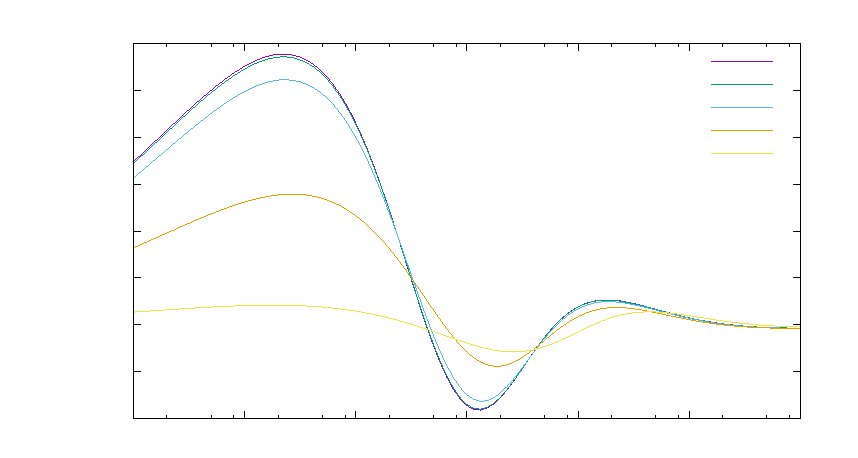
\includegraphics{img/cg1P}}%
    \gplfronttext
  \end{picture}%
\endgroup

	\caption{$c_{P,g}^{(1)}(\eta)$}
\end{subfigure}
\caption{next-to-leading order scaling functions $c_{k,g}^{(1)}(\eta,\xi)$ plotted as function of $\eta=s/(4m^2)-1$ for different values of $Q^2$ in units of $\si{\GeV^2}$ at $m=\SI{4.75}{\GeV}$ (i.e. different values of $\xi=Q^2/m^2$) }\label{fig:cg1}
\end{figure}

\pagebreak
\begin{figure}[ht!]
\centering
\begin{subfigure}[t]{\textwidth}
	% GNUPLOT: LaTeX picture with Postscript
\begingroup
  \makeatletter
  \providecommand\color[2][]{%
    \GenericError{(gnuplot) \space\space\space\@spaces}{%
      Package color not loaded in conjunction with
      terminal option `colourtext'%
    }{See the gnuplot documentation for explanation.%
    }{Either use 'blacktext' in gnuplot or load the package
      color.sty in LaTeX.}%
    \renewcommand\color[2][]{}%
  }%
  \providecommand\includegraphics[2][]{%
    \GenericError{(gnuplot) \space\space\space\@spaces}{%
      Package graphicx or graphics not loaded%
    }{See the gnuplot documentation for explanation.%
    }{The gnuplot epslatex terminal needs graphicx.sty or graphics.sty.}%
    \renewcommand\includegraphics[2][]{}%
  }%
  \providecommand\rotatebox[2]{#2}%
  \@ifundefined{ifGPcolor}{%
    \newif\ifGPcolor
    \GPcolorfalse
  }{}%
  \@ifundefined{ifGPblacktext}{%
    \newif\ifGPblacktext
    \GPblacktexttrue
  }{}%
  % define a \g@addto@macro without @ in the name:
  \let\gplgaddtomacro\g@addto@macro
  % define empty templates for all commands taking text:
  \gdef\gplbacktext{}%
  \gdef\gplfronttext{}%
  \makeatother
  \ifGPblacktext
    % no textcolor at all
    \def\colorrgb#1{}%
    \def\colorgray#1{}%
  \else
    % gray or color?
    \ifGPcolor
      \def\colorrgb#1{\color[rgb]{#1}}%
      \def\colorgray#1{\color[gray]{#1}}%
      \expandafter\def\csname LTw\endcsname{\color{white}}%
      \expandafter\def\csname LTb\endcsname{\color{black}}%
      \expandafter\def\csname LTa\endcsname{\color{black}}%
      \expandafter\def\csname LT0\endcsname{\color[rgb]{1,0,0}}%
      \expandafter\def\csname LT1\endcsname{\color[rgb]{0,1,0}}%
      \expandafter\def\csname LT2\endcsname{\color[rgb]{0,0,1}}%
      \expandafter\def\csname LT3\endcsname{\color[rgb]{1,0,1}}%
      \expandafter\def\csname LT4\endcsname{\color[rgb]{0,1,1}}%
      \expandafter\def\csname LT5\endcsname{\color[rgb]{1,1,0}}%
      \expandafter\def\csname LT6\endcsname{\color[rgb]{0,0,0}}%
      \expandafter\def\csname LT7\endcsname{\color[rgb]{1,0.3,0}}%
      \expandafter\def\csname LT8\endcsname{\color[rgb]{0.5,0.5,0.5}}%
    \else
      % gray
      \def\colorrgb#1{\color{black}}%
      \def\colorgray#1{\color[gray]{#1}}%
      \expandafter\def\csname LTw\endcsname{\color{white}}%
      \expandafter\def\csname LTb\endcsname{\color{black}}%
      \expandafter\def\csname LTa\endcsname{\color{black}}%
      \expandafter\def\csname LT0\endcsname{\color{black}}%
      \expandafter\def\csname LT1\endcsname{\color{black}}%
      \expandafter\def\csname LT2\endcsname{\color{black}}%
      \expandafter\def\csname LT3\endcsname{\color{black}}%
      \expandafter\def\csname LT4\endcsname{\color{black}}%
      \expandafter\def\csname LT5\endcsname{\color{black}}%
      \expandafter\def\csname LT6\endcsname{\color{black}}%
      \expandafter\def\csname LT7\endcsname{\color{black}}%
      \expandafter\def\csname LT8\endcsname{\color{black}}%
    \fi
  \fi
    \setlength{\unitlength}{0.0500bp}%
    \ifx\gptboxheight\undefined%
      \newlength{\gptboxheight}%
      \newlength{\gptboxwidth}%
      \newsavebox{\gptboxtext}%
    \fi%
    \setlength{\fboxrule}{0.5pt}%
    \setlength{\fboxsep}{1pt}%
\begin{picture}(7920.00,3628.80)%
    \gplgaddtomacro\gplbacktext{%
      \csname LTb\endcsname%
      \put(858,440){\makebox(0,0)[r]{\strut{}-0.20}}%
      \put(858,927){\makebox(0,0)[r]{\strut{}-0.15}}%
      \put(858,1415){\makebox(0,0)[r]{\strut{}-0.10}}%
      \put(858,1902){\makebox(0,0)[r]{\strut{}-0.05}}%
      \put(858,2389){\makebox(0,0)[r]{\strut{}0.00}}%
      \put(858,2877){\makebox(0,0)[r]{\strut{}0.05}}%
      \put(858,3364){\makebox(0,0)[r]{\strut{}0.10}}%
      \put(990,220){\makebox(0,0){\strut{}$0.001$}}%
      \put(2079,220){\makebox(0,0){\strut{}$0.01$}}%
      \put(3167,220){\makebox(0,0){\strut{}$0.1$}}%
      \put(4256,220){\makebox(0,0){\strut{}$1$}}%
      \put(5345,220){\makebox(0,0){\strut{}$10$}}%
      \put(6433,220){\makebox(0,0){\strut{}$100$}}%
      \put(7522,220){\makebox(0,0){\strut{}$1000$}}%
    }%
    \gplgaddtomacro\gplfronttext{%
      \csname LTb\endcsname%
      \put(1122,1493){\makebox(0,0)[l]{\strut{}$Q^2=10^{-2}$}}%
      \csname LTb\endcsname%
      \put(1122,1273){\makebox(0,0)[l]{\strut{}$Q^2=10^0$}}%
      \csname LTb\endcsname%
      \put(1122,1053){\makebox(0,0)[l]{\strut{}$Q^2=10^1$}}%
      \csname LTb\endcsname%
      \put(1122,833){\makebox(0,0)[l]{\strut{}$Q^2=10^2$}}%
      \csname LTb\endcsname%
      \put(1122,613){\makebox(0,0)[l]{\strut{}$Q^2=10^3$}}%
    }%
    \gplbacktext
    \put(0,0){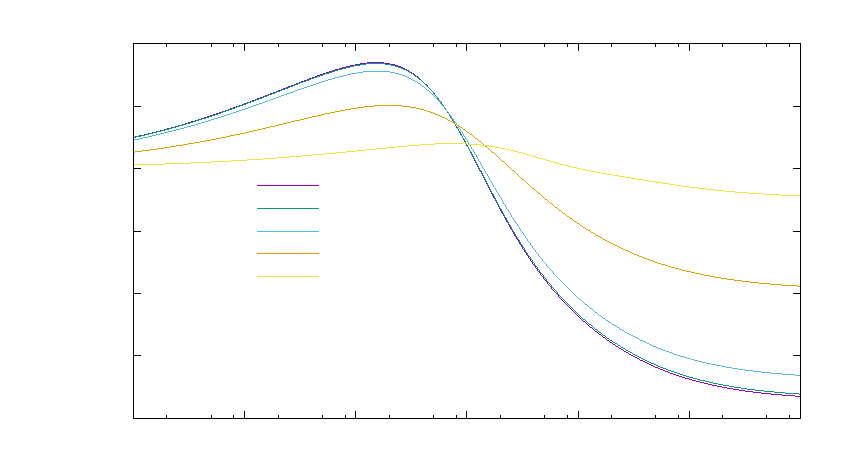
\includegraphics{img/cgBarF1T}}%
    \gplfronttext
  \end{picture}%
\endgroup

	\caption{$\bar c_{T,g}^{F,(1)}(\eta)$}
\end{subfigure}\\%
\begin{subfigure}[t]{\textwidth}
	% GNUPLOT: LaTeX picture with Postscript
\begingroup
  \makeatletter
  \providecommand\color[2][]{%
    \GenericError{(gnuplot) \space\space\space\@spaces}{%
      Package color not loaded in conjunction with
      terminal option `colourtext'%
    }{See the gnuplot documentation for explanation.%
    }{Either use 'blacktext' in gnuplot or load the package
      color.sty in LaTeX.}%
    \renewcommand\color[2][]{}%
  }%
  \providecommand\includegraphics[2][]{%
    \GenericError{(gnuplot) \space\space\space\@spaces}{%
      Package graphicx or graphics not loaded%
    }{See the gnuplot documentation for explanation.%
    }{The gnuplot epslatex terminal needs graphicx.sty or graphics.sty.}%
    \renewcommand\includegraphics[2][]{}%
  }%
  \providecommand\rotatebox[2]{#2}%
  \@ifundefined{ifGPcolor}{%
    \newif\ifGPcolor
    \GPcolorfalse
  }{}%
  \@ifundefined{ifGPblacktext}{%
    \newif\ifGPblacktext
    \GPblacktexttrue
  }{}%
  % define a \g@addto@macro without @ in the name:
  \let\gplgaddtomacro\g@addto@macro
  % define empty templates for all commands taking text:
  \gdef\gplbacktext{}%
  \gdef\gplfronttext{}%
  \makeatother
  \ifGPblacktext
    % no textcolor at all
    \def\colorrgb#1{}%
    \def\colorgray#1{}%
  \else
    % gray or color?
    \ifGPcolor
      \def\colorrgb#1{\color[rgb]{#1}}%
      \def\colorgray#1{\color[gray]{#1}}%
      \expandafter\def\csname LTw\endcsname{\color{white}}%
      \expandafter\def\csname LTb\endcsname{\color{black}}%
      \expandafter\def\csname LTa\endcsname{\color{black}}%
      \expandafter\def\csname LT0\endcsname{\color[rgb]{1,0,0}}%
      \expandafter\def\csname LT1\endcsname{\color[rgb]{0,1,0}}%
      \expandafter\def\csname LT2\endcsname{\color[rgb]{0,0,1}}%
      \expandafter\def\csname LT3\endcsname{\color[rgb]{1,0,1}}%
      \expandafter\def\csname LT4\endcsname{\color[rgb]{0,1,1}}%
      \expandafter\def\csname LT5\endcsname{\color[rgb]{1,1,0}}%
      \expandafter\def\csname LT6\endcsname{\color[rgb]{0,0,0}}%
      \expandafter\def\csname LT7\endcsname{\color[rgb]{1,0.3,0}}%
      \expandafter\def\csname LT8\endcsname{\color[rgb]{0.5,0.5,0.5}}%
    \else
      % gray
      \def\colorrgb#1{\color{black}}%
      \def\colorgray#1{\color[gray]{#1}}%
      \expandafter\def\csname LTw\endcsname{\color{white}}%
      \expandafter\def\csname LTb\endcsname{\color{black}}%
      \expandafter\def\csname LTa\endcsname{\color{black}}%
      \expandafter\def\csname LT0\endcsname{\color{black}}%
      \expandafter\def\csname LT1\endcsname{\color{black}}%
      \expandafter\def\csname LT2\endcsname{\color{black}}%
      \expandafter\def\csname LT3\endcsname{\color{black}}%
      \expandafter\def\csname LT4\endcsname{\color{black}}%
      \expandafter\def\csname LT5\endcsname{\color{black}}%
      \expandafter\def\csname LT6\endcsname{\color{black}}%
      \expandafter\def\csname LT7\endcsname{\color{black}}%
      \expandafter\def\csname LT8\endcsname{\color{black}}%
    \fi
  \fi
    \setlength{\unitlength}{0.0500bp}%
    \ifx\gptboxheight\undefined%
      \newlength{\gptboxheight}%
      \newlength{\gptboxwidth}%
      \newsavebox{\gptboxtext}%
    \fi%
    \setlength{\fboxrule}{0.5pt}%
    \setlength{\fboxsep}{1pt}%
\begin{picture}(7920.00,4082.40)%
    \gplgaddtomacro\gplbacktext{%
      \csname LTb\endcsname%
      \put(990,220){\makebox(0,0)[r]{\strut{}-0.015}}%
      \put(990,940){\makebox(0,0)[r]{\strut{}-0.010}}%
      \put(990,1659){\makebox(0,0)[r]{\strut{}-0.005}}%
      \put(990,2379){\makebox(0,0)[r]{\strut{}0.000}}%
      \put(990,3098){\makebox(0,0)[r]{\strut{}0.005}}%
      \put(990,3818){\makebox(0,0)[r]{\strut{}0.010}}%
      \put(1122,0){\makebox(0,0){\strut{}$0.001$}}%
      \put(2189,0){\makebox(0,0){\strut{}$0.01$}}%
      \put(3255,0){\makebox(0,0){\strut{}$0.1$}}%
      \put(4322,0){\makebox(0,0){\strut{}$1$}}%
      \put(5389,0){\makebox(0,0){\strut{}$10$}}%
      \put(6455,0){\makebox(0,0){\strut{}$100$}}%
      \put(7522,0){\makebox(0,0){\strut{}$1000$}}%
      \put(1250,472){\makebox(0,0)[l]{\strut{}(b) $\bar c_{L,g}^{F,(1)}(\eta)$}}%
    }%
    \gplgaddtomacro\gplfronttext{%
      \csname LTb\endcsname%
      \put(5611,3645){\makebox(0,0)[l]{\strut{}$Q^2=10^{-2}$}}%
      \csname LTb\endcsname%
      \put(5611,3425){\makebox(0,0)[l]{\strut{}$Q^2=10^0$}}%
      \csname LTb\endcsname%
      \put(5611,3205){\makebox(0,0)[l]{\strut{}$Q^2=10^1$}}%
      \csname LTb\endcsname%
      \put(5611,2985){\makebox(0,0)[l]{\strut{}$Q^2=10^2$}}%
      \csname LTb\endcsname%
      \put(5611,2765){\makebox(0,0)[l]{\strut{}$Q^2=10^3$}}%
    }%
    \gplbacktext
    \put(0,0){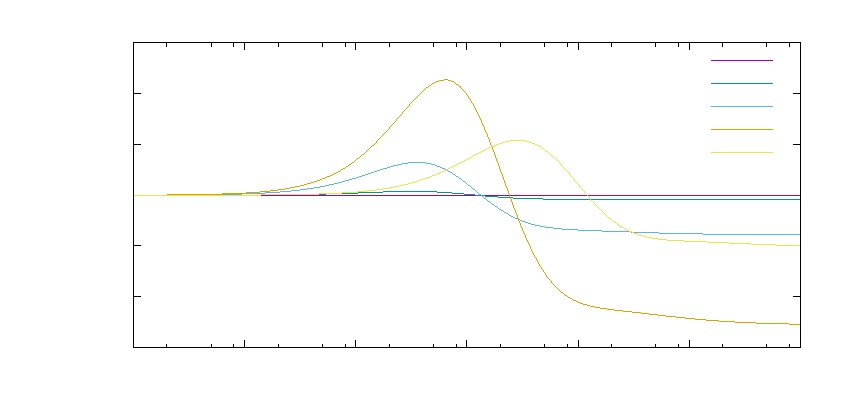
\includegraphics{img/cgBarF1L}}%
    \gplfronttext
  \end{picture}%
\endgroup

	\caption{$\bar c_{L,g}^{F,(1)}(\eta)$}
\end{subfigure}\\%
\begin{subfigure}[t]{\textwidth}
	% GNUPLOT: LaTeX picture with Postscript
\begingroup
  \makeatletter
  \providecommand\color[2][]{%
    \GenericError{(gnuplot) \space\space\space\@spaces}{%
      Package color not loaded in conjunction with
      terminal option `colourtext'%
    }{See the gnuplot documentation for explanation.%
    }{Either use 'blacktext' in gnuplot or load the package
      color.sty in LaTeX.}%
    \renewcommand\color[2][]{}%
  }%
  \providecommand\includegraphics[2][]{%
    \GenericError{(gnuplot) \space\space\space\@spaces}{%
      Package graphicx or graphics not loaded%
    }{See the gnuplot documentation for explanation.%
    }{The gnuplot epslatex terminal needs graphicx.sty or graphics.sty.}%
    \renewcommand\includegraphics[2][]{}%
  }%
  \providecommand\rotatebox[2]{#2}%
  \@ifundefined{ifGPcolor}{%
    \newif\ifGPcolor
    \GPcolorfalse
  }{}%
  \@ifundefined{ifGPblacktext}{%
    \newif\ifGPblacktext
    \GPblacktexttrue
  }{}%
  % define a \g@addto@macro without @ in the name:
  \let\gplgaddtomacro\g@addto@macro
  % define empty templates for all commands taking text:
  \gdef\gplbacktext{}%
  \gdef\gplfronttext{}%
  \makeatother
  \ifGPblacktext
    % no textcolor at all
    \def\colorrgb#1{}%
    \def\colorgray#1{}%
  \else
    % gray or color?
    \ifGPcolor
      \def\colorrgb#1{\color[rgb]{#1}}%
      \def\colorgray#1{\color[gray]{#1}}%
      \expandafter\def\csname LTw\endcsname{\color{white}}%
      \expandafter\def\csname LTb\endcsname{\color{black}}%
      \expandafter\def\csname LTa\endcsname{\color{black}}%
      \expandafter\def\csname LT0\endcsname{\color[rgb]{1,0,0}}%
      \expandafter\def\csname LT1\endcsname{\color[rgb]{0,1,0}}%
      \expandafter\def\csname LT2\endcsname{\color[rgb]{0,0,1}}%
      \expandafter\def\csname LT3\endcsname{\color[rgb]{1,0,1}}%
      \expandafter\def\csname LT4\endcsname{\color[rgb]{0,1,1}}%
      \expandafter\def\csname LT5\endcsname{\color[rgb]{1,1,0}}%
      \expandafter\def\csname LT6\endcsname{\color[rgb]{0,0,0}}%
      \expandafter\def\csname LT7\endcsname{\color[rgb]{1,0.3,0}}%
      \expandafter\def\csname LT8\endcsname{\color[rgb]{0.5,0.5,0.5}}%
    \else
      % gray
      \def\colorrgb#1{\color{black}}%
      \def\colorgray#1{\color[gray]{#1}}%
      \expandafter\def\csname LTw\endcsname{\color{white}}%
      \expandafter\def\csname LTb\endcsname{\color{black}}%
      \expandafter\def\csname LTa\endcsname{\color{black}}%
      \expandafter\def\csname LT0\endcsname{\color{black}}%
      \expandafter\def\csname LT1\endcsname{\color{black}}%
      \expandafter\def\csname LT2\endcsname{\color{black}}%
      \expandafter\def\csname LT3\endcsname{\color{black}}%
      \expandafter\def\csname LT4\endcsname{\color{black}}%
      \expandafter\def\csname LT5\endcsname{\color{black}}%
      \expandafter\def\csname LT6\endcsname{\color{black}}%
      \expandafter\def\csname LT7\endcsname{\color{black}}%
      \expandafter\def\csname LT8\endcsname{\color{black}}%
    \fi
  \fi
    \setlength{\unitlength}{0.0500bp}%
    \ifx\gptboxheight\undefined%
      \newlength{\gptboxheight}%
      \newlength{\gptboxwidth}%
      \newsavebox{\gptboxtext}%
    \fi%
    \setlength{\fboxrule}{0.5pt}%
    \setlength{\fboxsep}{1pt}%
\begin{picture}(7920.00,4082.40)%
    \gplgaddtomacro\gplbacktext{%
      \csname LTb\endcsname%
      \put(990,220){\makebox(0,0)[r]{\strut{} -0.04}}%
      \put(990,580){\makebox(0,0)[r]{\strut{} -0.03}}%
      \put(990,940){\makebox(0,0)[r]{\strut{} -0.02}}%
      \put(990,1299){\makebox(0,0)[r]{\strut{} -0.01}}%
      \put(990,1659){\makebox(0,0)[r]{\strut{} 0.00}}%
      \put(990,2019){\makebox(0,0)[r]{\strut{} 0.01}}%
      \put(990,2379){\makebox(0,0)[r]{\strut{} 0.02}}%
      \put(990,2739){\makebox(0,0)[r]{\strut{} 0.03}}%
      \put(990,3098){\makebox(0,0)[r]{\strut{} 0.04}}%
      \put(990,3458){\makebox(0,0)[r]{\strut{} 0.05}}%
      \put(990,3818){\makebox(0,0)[r]{\strut{} 0.06}}%
      \put(1122,0){\makebox(0,0){\strut{}$0.001$}}%
      \put(2189,0){\makebox(0,0){\strut{}$0.01$}}%
      \put(3255,0){\makebox(0,0){\strut{}$0.1$}}%
      \put(4322,0){\makebox(0,0){\strut{}$1$}}%
      \put(5389,0){\makebox(0,0){\strut{}$10$}}%
      \put(6455,0){\makebox(0,0){\strut{}$100$}}%
      \put(7522,0){\makebox(0,0){\strut{}$1000$}}%
      \put(1250,472){\makebox(0,0)[l]{\strut{}(c) $\bar c_{P,g}^{F,(1)}(\eta)$}}%
    }%
    \gplgaddtomacro\gplfronttext{%
      \csname LTb\endcsname%
      \put(5611,3645){\makebox(0,0)[l]{\strut{}$Q^2=10^{-2}$}}%
      \csname LTb\endcsname%
      \put(5611,3425){\makebox(0,0)[l]{\strut{}$Q^2=10^0$}}%
      \csname LTb\endcsname%
      \put(5611,3205){\makebox(0,0)[l]{\strut{}$Q^2=10^1$}}%
      \csname LTb\endcsname%
      \put(5611,2985){\makebox(0,0)[l]{\strut{}$Q^2=10^2$}}%
      \csname LTb\endcsname%
      \put(5611,2765){\makebox(0,0)[l]{\strut{}$Q^2=10^3$}}%
    }%
    \gplbacktext
    \put(0,0){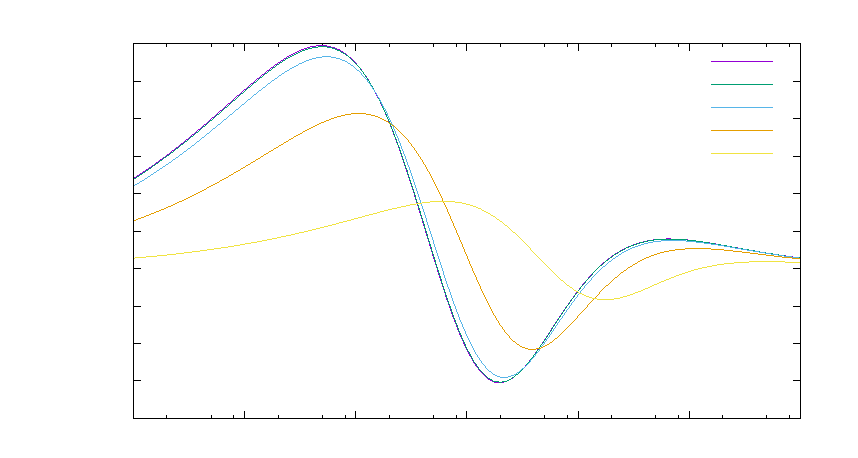
\includegraphics{img/cgBarF1P}}%
    \gplfronttext
  \end{picture}%
\endgroup

	\caption{$\bar c_{P,g}^{F,(1)}(\eta)$}
\end{subfigure}
\caption{next-to-leading order scaling functions $\bar c_{k,g}^{F,(1)}(\eta,\xi)$ plotted as function of $\eta=s/(4m^2)-1$ for different values of $Q^2$ in units of $\si{\GeV^2}$ at $m=\SI{4.75}{\GeV}$ (i.e. different values of $\xi=Q^2/m^2$) and $n_{lf}=4$ }\label{fig:cg1}
\end{figure}

\pagebreak
\begin{figure}[ht!]
\centering
\begin{subfigure}[t]{\textwidth}
	% GNUPLOT: LaTeX picture with Postscript
\begingroup
  \makeatletter
  \providecommand\color[2][]{%
    \GenericError{(gnuplot) \space\space\space\@spaces}{%
      Package color not loaded in conjunction with
      terminal option `colourtext'%
    }{See the gnuplot documentation for explanation.%
    }{Either use 'blacktext' in gnuplot or load the package
      color.sty in LaTeX.}%
    \renewcommand\color[2][]{}%
  }%
  \providecommand\includegraphics[2][]{%
    \GenericError{(gnuplot) \space\space\space\@spaces}{%
      Package graphicx or graphics not loaded%
    }{See the gnuplot documentation for explanation.%
    }{The gnuplot epslatex terminal needs graphicx.sty or graphics.sty.}%
    \renewcommand\includegraphics[2][]{}%
  }%
  \providecommand\rotatebox[2]{#2}%
  \@ifundefined{ifGPcolor}{%
    \newif\ifGPcolor
    \GPcolorfalse
  }{}%
  \@ifundefined{ifGPblacktext}{%
    \newif\ifGPblacktext
    \GPblacktexttrue
  }{}%
  % define a \g@addto@macro without @ in the name:
  \let\gplgaddtomacro\g@addto@macro
  % define empty templates for all commands taking text:
  \gdef\gplbacktext{}%
  \gdef\gplfronttext{}%
  \makeatother
  \ifGPblacktext
    % no textcolor at all
    \def\colorrgb#1{}%
    \def\colorgray#1{}%
  \else
    % gray or color?
    \ifGPcolor
      \def\colorrgb#1{\color[rgb]{#1}}%
      \def\colorgray#1{\color[gray]{#1}}%
      \expandafter\def\csname LTw\endcsname{\color{white}}%
      \expandafter\def\csname LTb\endcsname{\color{black}}%
      \expandafter\def\csname LTa\endcsname{\color{black}}%
      \expandafter\def\csname LT0\endcsname{\color[rgb]{1,0,0}}%
      \expandafter\def\csname LT1\endcsname{\color[rgb]{0,1,0}}%
      \expandafter\def\csname LT2\endcsname{\color[rgb]{0,0,1}}%
      \expandafter\def\csname LT3\endcsname{\color[rgb]{1,0,1}}%
      \expandafter\def\csname LT4\endcsname{\color[rgb]{0,1,1}}%
      \expandafter\def\csname LT5\endcsname{\color[rgb]{1,1,0}}%
      \expandafter\def\csname LT6\endcsname{\color[rgb]{0,0,0}}%
      \expandafter\def\csname LT7\endcsname{\color[rgb]{1,0.3,0}}%
      \expandafter\def\csname LT8\endcsname{\color[rgb]{0.5,0.5,0.5}}%
    \else
      % gray
      \def\colorrgb#1{\color{black}}%
      \def\colorgray#1{\color[gray]{#1}}%
      \expandafter\def\csname LTw\endcsname{\color{white}}%
      \expandafter\def\csname LTb\endcsname{\color{black}}%
      \expandafter\def\csname LTa\endcsname{\color{black}}%
      \expandafter\def\csname LT0\endcsname{\color{black}}%
      \expandafter\def\csname LT1\endcsname{\color{black}}%
      \expandafter\def\csname LT2\endcsname{\color{black}}%
      \expandafter\def\csname LT3\endcsname{\color{black}}%
      \expandafter\def\csname LT4\endcsname{\color{black}}%
      \expandafter\def\csname LT5\endcsname{\color{black}}%
      \expandafter\def\csname LT6\endcsname{\color{black}}%
      \expandafter\def\csname LT7\endcsname{\color{black}}%
      \expandafter\def\csname LT8\endcsname{\color{black}}%
    \fi
  \fi
    \setlength{\unitlength}{0.0500bp}%
    \ifx\gptboxheight\undefined%
      \newlength{\gptboxheight}%
      \newlength{\gptboxwidth}%
      \newsavebox{\gptboxtext}%
    \fi%
    \setlength{\fboxrule}{0.5pt}%
    \setlength{\fboxsep}{1pt}%
\begin{picture}(7920.00,4082.40)%
    \gplgaddtomacro\gplbacktext{%
      \csname LTb\endcsname%
      \put(726,220){\makebox(0,0)[r]{\strut{}0.00}}%
      \put(726,580){\makebox(0,0)[r]{\strut{}0.01}}%
      \put(726,940){\makebox(0,0)[r]{\strut{}0.02}}%
      \put(726,1299){\makebox(0,0)[r]{\strut{}0.03}}%
      \put(726,1659){\makebox(0,0)[r]{\strut{}0.04}}%
      \put(726,2019){\makebox(0,0)[r]{\strut{}0.05}}%
      \put(726,2379){\makebox(0,0)[r]{\strut{}0.06}}%
      \put(726,2739){\makebox(0,0)[r]{\strut{}0.07}}%
      \put(726,3098){\makebox(0,0)[r]{\strut{}0.08}}%
      \put(726,3458){\makebox(0,0)[r]{\strut{}0.09}}%
      \put(726,3818){\makebox(0,0)[r]{\strut{}0.10}}%
      \put(858,0){\makebox(0,0){\strut{}$0.001$}}%
      \put(1969,0){\makebox(0,0){\strut{}$0.01$}}%
      \put(3079,0){\makebox(0,0){\strut{}$0.1$}}%
      \put(4190,0){\makebox(0,0){\strut{}$1$}}%
      \put(5301,0){\makebox(0,0){\strut{}$10$}}%
      \put(6411,0){\makebox(0,0){\strut{}$100$}}%
      \put(7522,0){\makebox(0,0){\strut{}$1000$}}%
      \put(991,3458){\makebox(0,0)[l]{\strut{}(a) $\bar c_{T,g}^{R,(1)}(\eta)$}}%
    }%
    \gplgaddtomacro\gplfronttext{%
      \csname LTb\endcsname%
      \put(5611,3645){\makebox(0,0)[l]{\strut{}$Q^2=10^{-2}$}}%
      \csname LTb\endcsname%
      \put(5611,3425){\makebox(0,0)[l]{\strut{}$Q^2=10^0$}}%
      \csname LTb\endcsname%
      \put(5611,3205){\makebox(0,0)[l]{\strut{}$Q^2=10^1$}}%
      \csname LTb\endcsname%
      \put(5611,2985){\makebox(0,0)[l]{\strut{}$Q^2=10^2$}}%
      \csname LTb\endcsname%
      \put(5611,2765){\makebox(0,0)[l]{\strut{}$Q^2=10^3$}}%
    }%
    \gplbacktext
    \put(0,0){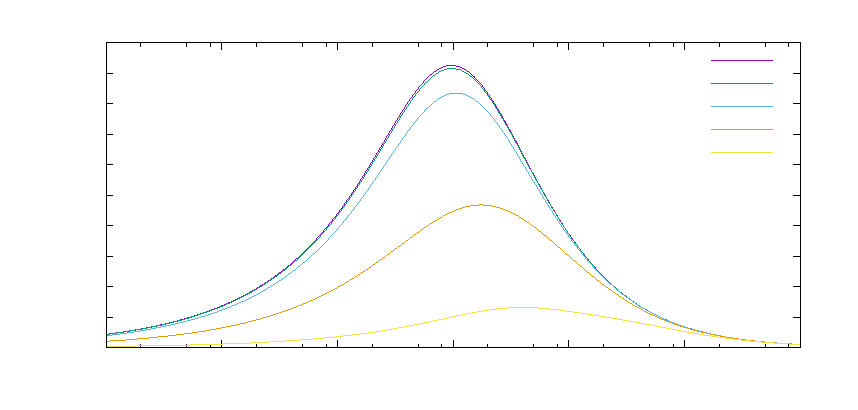
\includegraphics{img/cgBarR1T}}%
    \gplfronttext
  \end{picture}%
\endgroup

	\caption{$\bar c_{T,g}^{R,(1)}(\eta)$}
\end{subfigure}\\%
\begin{subfigure}[t]{\textwidth}
	% GNUPLOT: LaTeX picture with Postscript
\begingroup
  \makeatletter
  \providecommand\color[2][]{%
    \GenericError{(gnuplot) \space\space\space\@spaces}{%
      Package color not loaded in conjunction with
      terminal option `colourtext'%
    }{See the gnuplot documentation for explanation.%
    }{Either use 'blacktext' in gnuplot or load the package
      color.sty in LaTeX.}%
    \renewcommand\color[2][]{}%
  }%
  \providecommand\includegraphics[2][]{%
    \GenericError{(gnuplot) \space\space\space\@spaces}{%
      Package graphicx or graphics not loaded%
    }{See the gnuplot documentation for explanation.%
    }{The gnuplot epslatex terminal needs graphicx.sty or graphics.sty.}%
    \renewcommand\includegraphics[2][]{}%
  }%
  \providecommand\rotatebox[2]{#2}%
  \@ifundefined{ifGPcolor}{%
    \newif\ifGPcolor
    \GPcolorfalse
  }{}%
  \@ifundefined{ifGPblacktext}{%
    \newif\ifGPblacktext
    \GPblacktexttrue
  }{}%
  % define a \g@addto@macro without @ in the name:
  \let\gplgaddtomacro\g@addto@macro
  % define empty templates for all commands taking text:
  \gdef\gplbacktext{}%
  \gdef\gplfronttext{}%
  \makeatother
  \ifGPblacktext
    % no textcolor at all
    \def\colorrgb#1{}%
    \def\colorgray#1{}%
  \else
    % gray or color?
    \ifGPcolor
      \def\colorrgb#1{\color[rgb]{#1}}%
      \def\colorgray#1{\color[gray]{#1}}%
      \expandafter\def\csname LTw\endcsname{\color{white}}%
      \expandafter\def\csname LTb\endcsname{\color{black}}%
      \expandafter\def\csname LTa\endcsname{\color{black}}%
      \expandafter\def\csname LT0\endcsname{\color[rgb]{1,0,0}}%
      \expandafter\def\csname LT1\endcsname{\color[rgb]{0,1,0}}%
      \expandafter\def\csname LT2\endcsname{\color[rgb]{0,0,1}}%
      \expandafter\def\csname LT3\endcsname{\color[rgb]{1,0,1}}%
      \expandafter\def\csname LT4\endcsname{\color[rgb]{0,1,1}}%
      \expandafter\def\csname LT5\endcsname{\color[rgb]{1,1,0}}%
      \expandafter\def\csname LT6\endcsname{\color[rgb]{0,0,0}}%
      \expandafter\def\csname LT7\endcsname{\color[rgb]{1,0.3,0}}%
      \expandafter\def\csname LT8\endcsname{\color[rgb]{0.5,0.5,0.5}}%
    \else
      % gray
      \def\colorrgb#1{\color{black}}%
      \def\colorgray#1{\color[gray]{#1}}%
      \expandafter\def\csname LTw\endcsname{\color{white}}%
      \expandafter\def\csname LTb\endcsname{\color{black}}%
      \expandafter\def\csname LTa\endcsname{\color{black}}%
      \expandafter\def\csname LT0\endcsname{\color{black}}%
      \expandafter\def\csname LT1\endcsname{\color{black}}%
      \expandafter\def\csname LT2\endcsname{\color{black}}%
      \expandafter\def\csname LT3\endcsname{\color{black}}%
      \expandafter\def\csname LT4\endcsname{\color{black}}%
      \expandafter\def\csname LT5\endcsname{\color{black}}%
      \expandafter\def\csname LT6\endcsname{\color{black}}%
      \expandafter\def\csname LT7\endcsname{\color{black}}%
      \expandafter\def\csname LT8\endcsname{\color{black}}%
    \fi
  \fi
    \setlength{\unitlength}{0.0500bp}%
    \ifx\gptboxheight\undefined%
      \newlength{\gptboxheight}%
      \newlength{\gptboxwidth}%
      \newsavebox{\gptboxtext}%
    \fi%
    \setlength{\fboxrule}{0.5pt}%
    \setlength{\fboxsep}{1pt}%
\begin{picture}(7920.00,3628.80)%
    \gplgaddtomacro\gplbacktext{%
      \csname LTb\endcsname%
      \put(858,440){\makebox(0,0)[r]{\strut{}0.000}}%
      \put(858,927){\makebox(0,0)[r]{\strut{}0.002}}%
      \put(858,1415){\makebox(0,0)[r]{\strut{}0.004}}%
      \put(858,1902){\makebox(0,0)[r]{\strut{}0.006}}%
      \put(858,2389){\makebox(0,0)[r]{\strut{}0.008}}%
      \put(858,2877){\makebox(0,0)[r]{\strut{}0.010}}%
      \put(858,3364){\makebox(0,0)[r]{\strut{}0.012}}%
      \put(990,220){\makebox(0,0){\strut{}$0.001$}}%
      \put(2079,220){\makebox(0,0){\strut{}$0.01$}}%
      \put(3167,220){\makebox(0,0){\strut{}$0.1$}}%
      \put(4256,220){\makebox(0,0){\strut{}$1$}}%
      \put(5345,220){\makebox(0,0){\strut{}$10$}}%
      \put(6433,220){\makebox(0,0){\strut{}$100$}}%
      \put(7522,220){\makebox(0,0){\strut{}$1000$}}%
    }%
    \gplgaddtomacro\gplfronttext{%
      \csname LTb\endcsname%
      \put(5611,3191){\makebox(0,0)[l]{\strut{}$Q^2=10^{-2}$}}%
      \csname LTb\endcsname%
      \put(5611,2971){\makebox(0,0)[l]{\strut{}$Q^2=10^0$}}%
      \csname LTb\endcsname%
      \put(5611,2751){\makebox(0,0)[l]{\strut{}$Q^2=10^1$}}%
      \csname LTb\endcsname%
      \put(5611,2531){\makebox(0,0)[l]{\strut{}$Q^2=10^2$}}%
      \csname LTb\endcsname%
      \put(5611,2311){\makebox(0,0)[l]{\strut{}$Q^2=10^3$}}%
    }%
    \gplbacktext
    \put(0,0){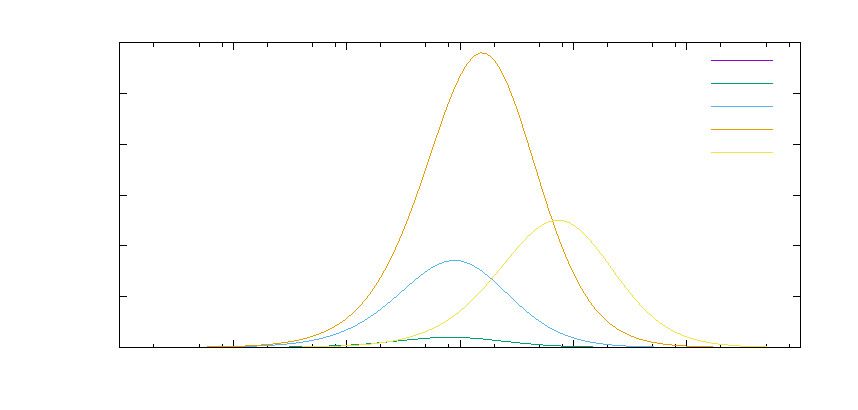
\includegraphics{img/cgBarR1L}}%
    \gplfronttext
  \end{picture}%
\endgroup

	\caption{$\bar c_{L,g}^{R,(1)}(\eta)$}
\end{subfigure}\\%
\begin{subfigure}[t]{\textwidth}
	% GNUPLOT: LaTeX picture with Postscript
\begingroup
  \makeatletter
  \providecommand\color[2][]{%
    \GenericError{(gnuplot) \space\space\space\@spaces}{%
      Package color not loaded in conjunction with
      terminal option `colourtext'%
    }{See the gnuplot documentation for explanation.%
    }{Either use 'blacktext' in gnuplot or load the package
      color.sty in LaTeX.}%
    \renewcommand\color[2][]{}%
  }%
  \providecommand\includegraphics[2][]{%
    \GenericError{(gnuplot) \space\space\space\@spaces}{%
      Package graphicx or graphics not loaded%
    }{See the gnuplot documentation for explanation.%
    }{The gnuplot epslatex terminal needs graphicx.sty or graphics.sty.}%
    \renewcommand\includegraphics[2][]{}%
  }%
  \providecommand\rotatebox[2]{#2}%
  \@ifundefined{ifGPcolor}{%
    \newif\ifGPcolor
    \GPcolorfalse
  }{}%
  \@ifundefined{ifGPblacktext}{%
    \newif\ifGPblacktext
    \GPblacktexttrue
  }{}%
  % define a \g@addto@macro without @ in the name:
  \let\gplgaddtomacro\g@addto@macro
  % define empty templates for all commands taking text:
  \gdef\gplbacktext{}%
  \gdef\gplfronttext{}%
  \makeatother
  \ifGPblacktext
    % no textcolor at all
    \def\colorrgb#1{}%
    \def\colorgray#1{}%
  \else
    % gray or color?
    \ifGPcolor
      \def\colorrgb#1{\color[rgb]{#1}}%
      \def\colorgray#1{\color[gray]{#1}}%
      \expandafter\def\csname LTw\endcsname{\color{white}}%
      \expandafter\def\csname LTb\endcsname{\color{black}}%
      \expandafter\def\csname LTa\endcsname{\color{black}}%
      \expandafter\def\csname LT0\endcsname{\color[rgb]{1,0,0}}%
      \expandafter\def\csname LT1\endcsname{\color[rgb]{0,1,0}}%
      \expandafter\def\csname LT2\endcsname{\color[rgb]{0,0,1}}%
      \expandafter\def\csname LT3\endcsname{\color[rgb]{1,0,1}}%
      \expandafter\def\csname LT4\endcsname{\color[rgb]{0,1,1}}%
      \expandafter\def\csname LT5\endcsname{\color[rgb]{1,1,0}}%
      \expandafter\def\csname LT6\endcsname{\color[rgb]{0,0,0}}%
      \expandafter\def\csname LT7\endcsname{\color[rgb]{1,0.3,0}}%
      \expandafter\def\csname LT8\endcsname{\color[rgb]{0.5,0.5,0.5}}%
    \else
      % gray
      \def\colorrgb#1{\color{black}}%
      \def\colorgray#1{\color[gray]{#1}}%
      \expandafter\def\csname LTw\endcsname{\color{white}}%
      \expandafter\def\csname LTb\endcsname{\color{black}}%
      \expandafter\def\csname LTa\endcsname{\color{black}}%
      \expandafter\def\csname LT0\endcsname{\color{black}}%
      \expandafter\def\csname LT1\endcsname{\color{black}}%
      \expandafter\def\csname LT2\endcsname{\color{black}}%
      \expandafter\def\csname LT3\endcsname{\color{black}}%
      \expandafter\def\csname LT4\endcsname{\color{black}}%
      \expandafter\def\csname LT5\endcsname{\color{black}}%
      \expandafter\def\csname LT6\endcsname{\color{black}}%
      \expandafter\def\csname LT7\endcsname{\color{black}}%
      \expandafter\def\csname LT8\endcsname{\color{black}}%
    \fi
  \fi
    \setlength{\unitlength}{0.0500bp}%
    \ifx\gptboxheight\undefined%
      \newlength{\gptboxheight}%
      \newlength{\gptboxwidth}%
      \newsavebox{\gptboxtext}%
    \fi%
    \setlength{\fboxrule}{0.5pt}%
    \setlength{\fboxsep}{1pt}%
\begin{picture}(7920.00,4082.40)%
    \gplgaddtomacro\gplbacktext{%
      \csname LTb\endcsname%
      \put(858,220){\makebox(0,0)[r]{\strut{}-0.02}}%
      \put(858,734){\makebox(0,0)[r]{\strut{}-0.01}}%
      \put(858,1248){\makebox(0,0)[r]{\strut{}0.00}}%
      \put(858,1762){\makebox(0,0)[r]{\strut{}0.01}}%
      \put(858,2276){\makebox(0,0)[r]{\strut{}0.02}}%
      \put(858,2790){\makebox(0,0)[r]{\strut{}0.03}}%
      \put(858,3304){\makebox(0,0)[r]{\strut{}0.04}}%
      \put(858,3818){\makebox(0,0)[r]{\strut{}0.05}}%
      \put(990,0){\makebox(0,0){\strut{}$0.001$}}%
      \put(2079,0){\makebox(0,0){\strut{}$0.01$}}%
      \put(3167,0){\makebox(0,0){\strut{}$0.1$}}%
      \put(4256,0){\makebox(0,0){\strut{}$1$}}%
      \put(5345,0){\makebox(0,0){\strut{}$10$}}%
      \put(6433,0){\makebox(0,0){\strut{}$100$}}%
      \put(7522,0){\makebox(0,0){\strut{}$1000$}}%
      \put(1121,3458){\makebox(0,0)[l]{\strut{}(c) $\bar c_{P,g}^{R,(1)}(\eta)$}}%
    }%
    \gplgaddtomacro\gplfronttext{%
      \csname LTb\endcsname%
      \put(5611,3645){\makebox(0,0)[l]{\strut{}$Q^2=10^{-2}$}}%
      \csname LTb\endcsname%
      \put(5611,3425){\makebox(0,0)[l]{\strut{}$Q^2=10^0$}}%
      \csname LTb\endcsname%
      \put(5611,3205){\makebox(0,0)[l]{\strut{}$Q^2=10^1$}}%
      \csname LTb\endcsname%
      \put(5611,2985){\makebox(0,0)[l]{\strut{}$Q^2=10^2$}}%
      \csname LTb\endcsname%
      \put(5611,2765){\makebox(0,0)[l]{\strut{}$Q^2=10^3$}}%
    }%
    \gplbacktext
    \put(0,0){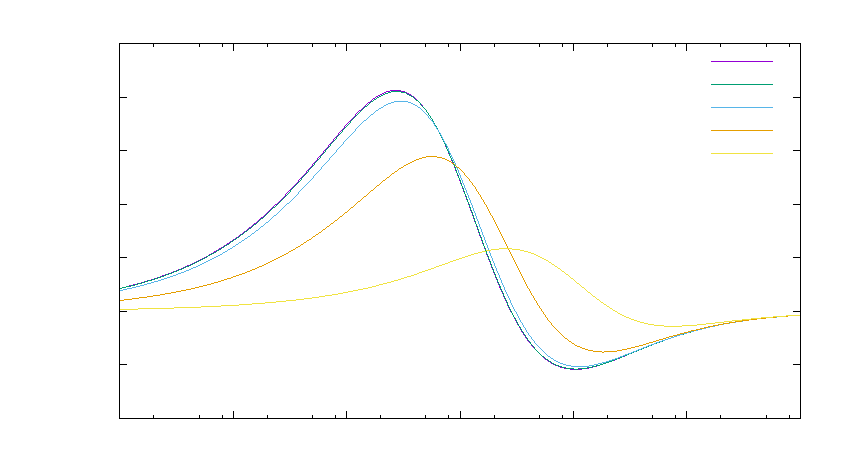
\includegraphics{img/cgBarR1P}}%
    \gplfronttext
  \end{picture}%
\endgroup

	\caption{$\bar c_{P,g}^{R,(1)}(\eta)$}
\end{subfigure}
\caption{next-to-leading order scaling functions $\bar c_{k,g}^{R,(1)}(\eta,\xi)$ plotted as function of $\eta=s/(4m^2)-1$ for different values of $Q^2$ in units of $\si{\GeV^2}$ at $m=\SI{4.75}{\GeV}$ (i.e. different values of $\xi=Q^2/m^2$) and $n_{lf}=4$ }\label{fig:cg1}
\end{figure}

\clearpage


\section{Hadronic Results}
\begin{frame}{Hadronic Results - Unpolarized vs. Polarized}
\begin{center}
unpolarized $\sim$ MSTW2008 $\leftrightarrow$ polarized $\sim$ DSSV2014\quad\,\,\,\\
\quad\quad\quad\iRef{Martin,Stirling,Thorne,Watt} $\leftrightarrow$ \iRef{de Florian,Sassot,Stratmann,Vogelsang}
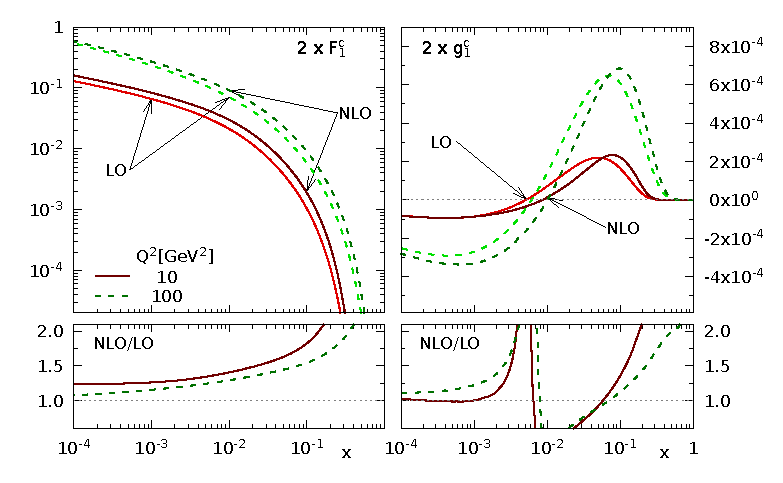
\includegraphics[width=.8\textwidth]{img/F1g1}
\end{center}
\end{frame}

\begin{frame}{Hadronic Results - PDF Uncertainties DSSV (I)}
\newcolumntype{w}{>{\centering\arraybackslash} m{.60\linewidth} }
\newcolumntype{n}{>{\centering\arraybackslash} m{.39\linewidth} }
\begin{tabular}{wn}
\begin{center}
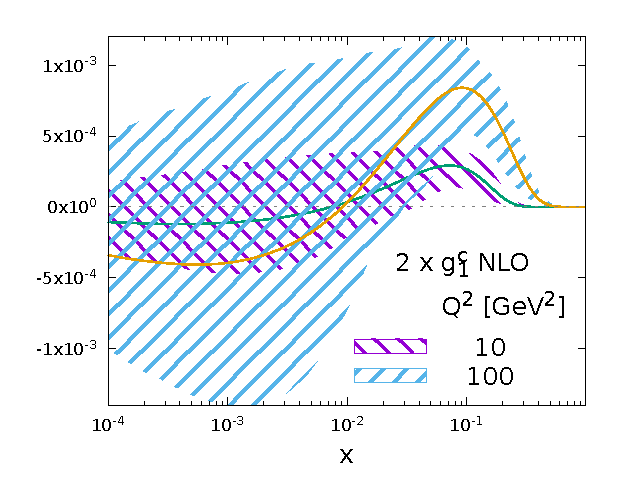
\includegraphics[width=.65\textwidth]{img/g1NLO-pdf}
\end{center} & 
\begin{itemize}
\item quark error band is small
\item sign unconstrained
\item gluon dominates (?)
\item default gluon is small
\end{itemize}
\end{tabular}
\end{frame}

\begin{frame}{Hadronic Results - PDF Uncertainties DSSV (II)}
\newcolumntype{w}{>{\centering\arraybackslash} m{.5\linewidth} }
\newcolumntype{n}{>{\centering\arraybackslash} m{.5\linewidth} }
\begin{tabular}{wn}
\begin{center}
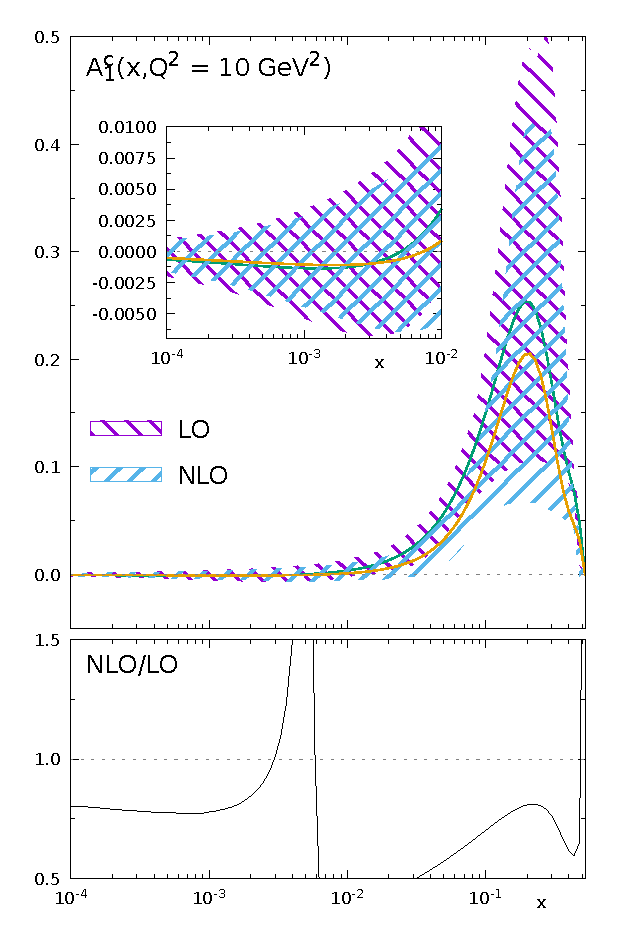
\includegraphics[height=.97\textheight]{img/A1-pdf}
\end{center} & 
\begin{itemize}
\item $A_1^c(x,Q^2) = \frac{g_1^c(x,Q^2)}{F_1^c(x,Q^2)}$
\item error band are only due to DSSV uncertainties (no correlations!)
\invisible{
\item sign unconstrained
\item need measurement of $\mathcal O(10^{-3})$
\item NLO $\lessapprox$ LO}
\end{itemize}
\end{tabular}
\end{frame}
\begin{frame}{Hadronic Results - PDF Uncertainties DSSV (II)}
\newcolumntype{w}{>{\centering\arraybackslash} m{.5\linewidth} }
\newcolumntype{n}{>{\centering\arraybackslash} m{.5\linewidth} }
\begin{tabular}{wn}
\begin{center}
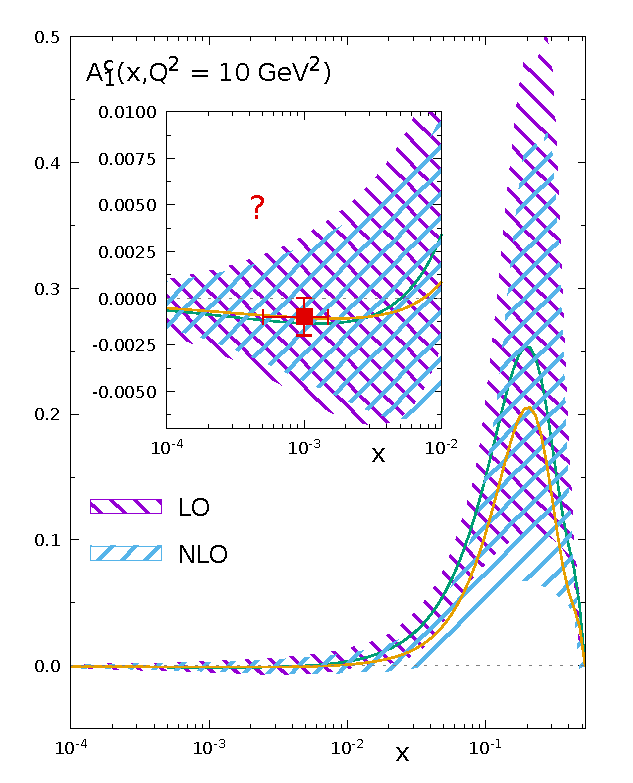
\includegraphics[height=.97\textheight]{img/A1-pdf-data}
\end{center} & 
\begin{itemize}
\item $A_1^c(x,Q^2) = \frac{g_1^c(x,Q^2)}{F_1^c(x,Q^2)}$
\item error band are only due to DSSV uncertainties (no correlations!)
\item sign unconstrained
\item need measurement of $\mathcal O(10^{-3})$
\item NLO $\lessapprox$ LO
\end{itemize}
\end{tabular}
\end{frame}

\begin{frame}{Hadronic Results - Scale Uncertainties (I)}
\begin{center}
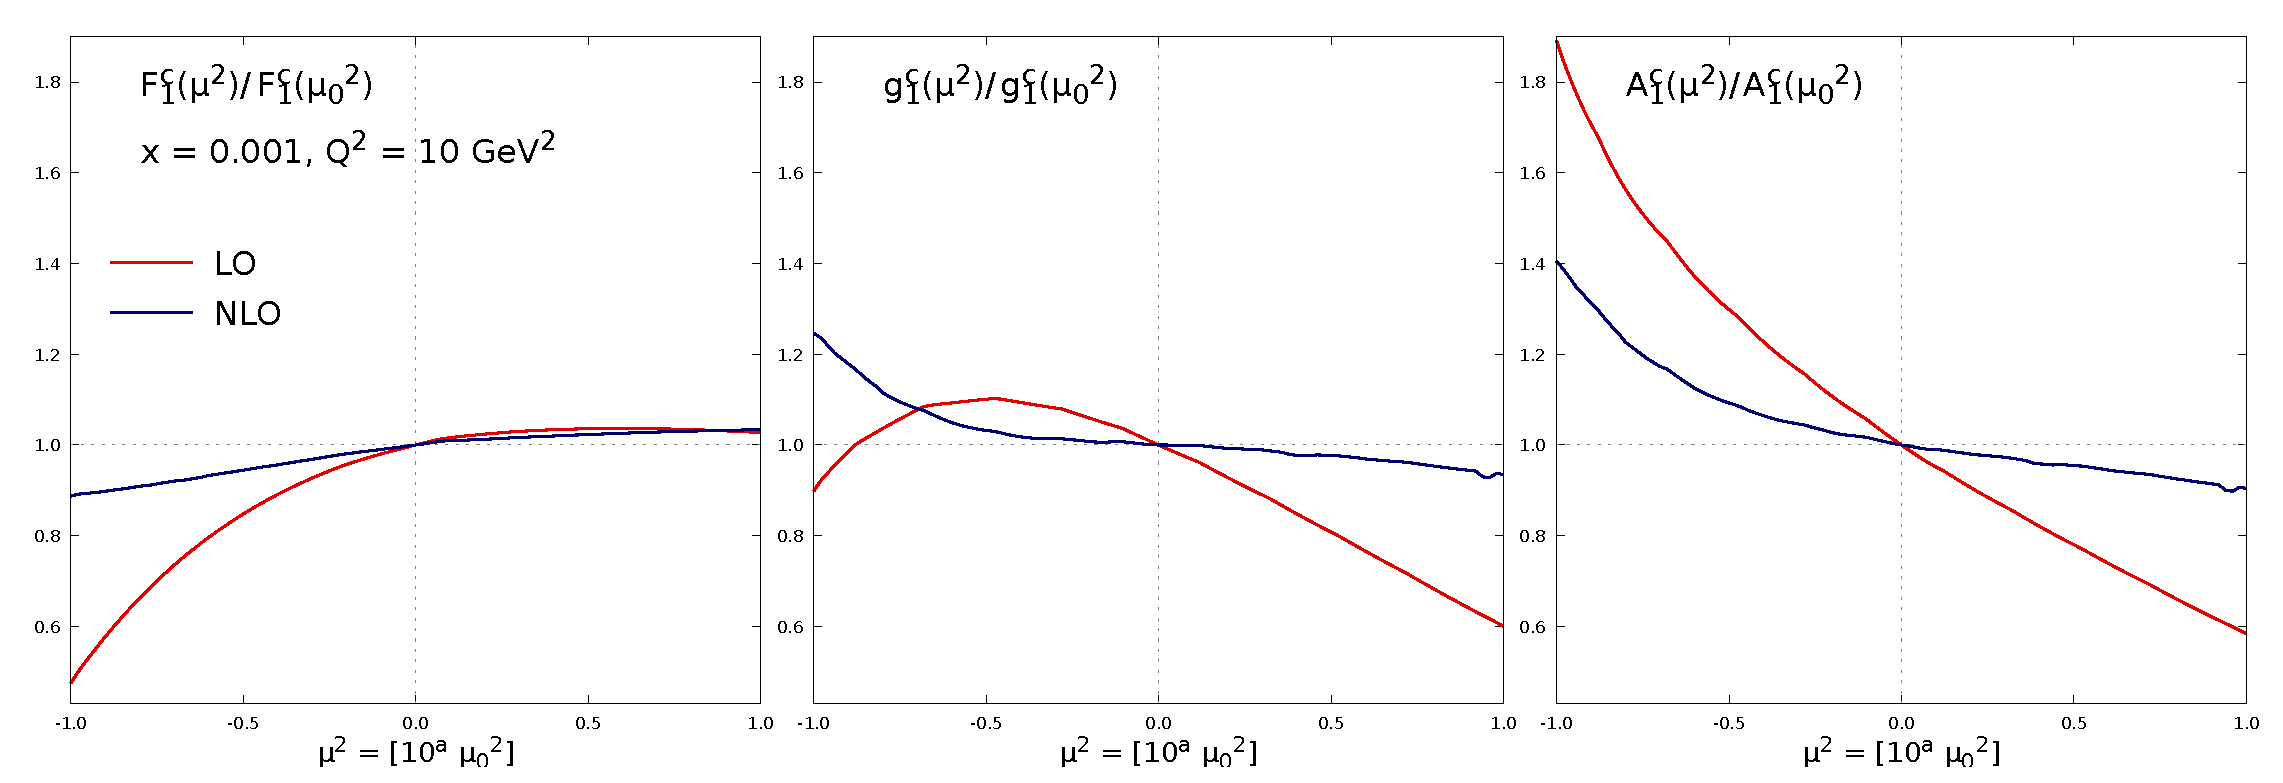
\includegraphics[width=\textwidth]{img/F1g1A1-mu2}
\end{center}
\[\mu_F^2 = \mu_R^2 = 10^a\mu_0^2\,\text{with}\,\mu_0^2=4m^2+Q^2\]
\end{frame}

\begin{frame}{Hadronic Results - Scale Uncertainties (II)}
\begin{center}
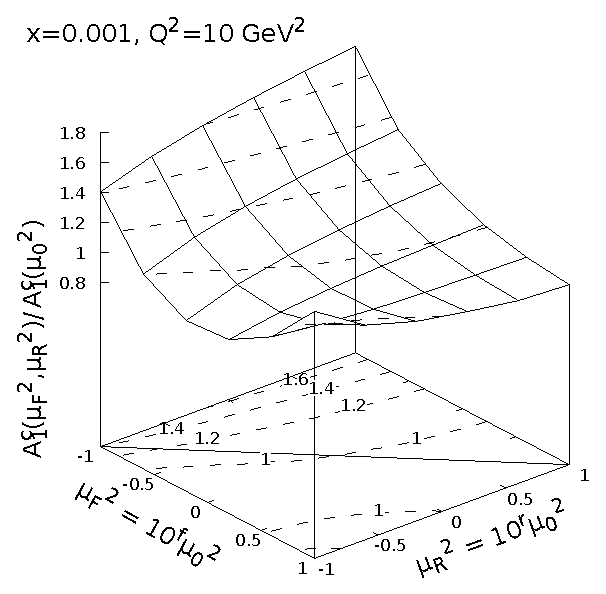
\includegraphics[width=.48\textwidth]{img/A1-muF2-muR2-x_3-q2_1}
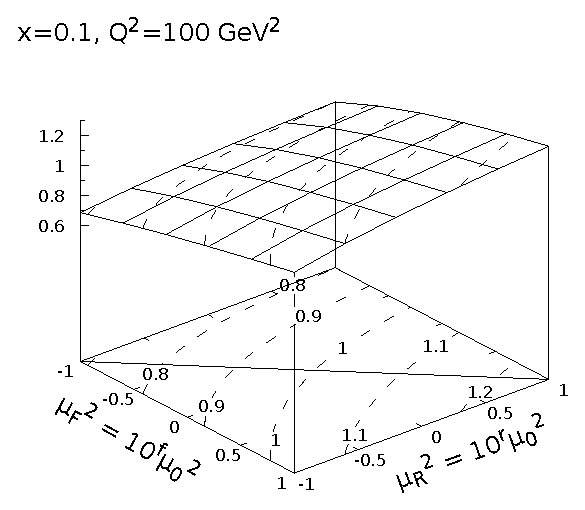
\includegraphics[width=.48\textwidth]{img/A1-muF2-muR2-x_1-q2_2}
\end{center}
\[\mu_0^2=4m^2+Q^2\]
\end{frame}


\section{Outlook}
\begin{frame}{Outlook}
\begin{itemize}
\item inclusive distributions: $\DeriveF{{p_{T,\PaQ}}}{g_1},\DeriveF{{y_{\PaQ}}}{g_1}$
\item correlated distributions: $\DeriveF{{M_{\PQ\PaQ}^2}}{g_1}, \DeriveF{\phi_{\PQ\PaQ}}{g_1}$
\item<2-> full neutral current (NC) contributions: $F_3^{\PZ\Pgg}, g_4^{\PZ\Pgg}, g_5^{\PZ\Pgg}$ and $F_2^{\PZ}, F_L^{\PZ}, g_1^{\PZ}$
\item<2-> distributions of full NC structure functions: $\DeriveF{p_{T,\PaQ}}{g_1^{NC}},\DeriveF{{M_{\PQ\PaQ}^2}}{g_1^{NC}}$
\end{itemize}

\uncover<3->{\vspace{1cm}
\setbeamercolor{thanks}{bg=UniRot,fg=white}
\begin{beamercolorbox}[ht=2.5ex,dp=1ex,center]{thanks}
Thank you for your attention!
\end{beamercolorbox}}
\end{frame}

\section*{Backup}
\begin{frame}{Backup: Hadronic Results - Mass Variation}
\begin{center}
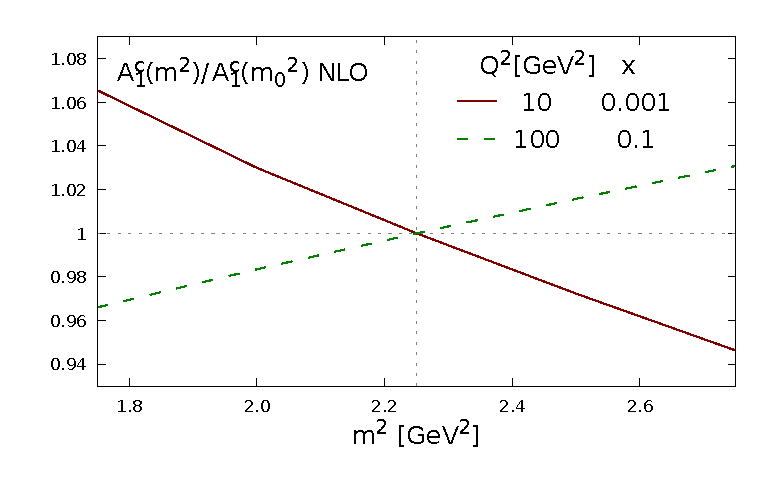
\includegraphics[width=.75\textwidth]{img/A1-m2}
\end{center}
\[m_0=\SI{1.5}{\GeV}\]
\end{frame}


\end{document}
